\chapter{Evaluations}
%-----------------------------------------------------------------------------------------------------------------------------------------------------------------
\section{Kaa}
\label{sec:kaa}
%Mention kodiak, general structure of program, difference between kaa and dynamic.
%
We evaluate the efficacy of our dynamic parallelotope bundle strategies with our tool, \emph{Kaa} .
%
Kaa is written in Python and relies on several modules to perform reachable set computation.
\begin{description}
  \item[Numpy:] The \emph{Numpy} module is used to do all matrix computations, such as matrix multiplication and matrix inversions. It is also used to efficiently solve systems of linear equations, especially those which arise from converting from half-space representation to generator representation (See Section \ref{sec:parallelotope}), and execute the Least Squares routine required to compute the solution to Problem \ref{eq:least_squares}.
  %
  \item[Sympy:] The \emph{Sympy} module is used to do all symbolic computations. The polynomials which result from performing the $\Lambda_i \cdot f(x)$ in Equation \ref{eq:maxalpha} are all simplified and encapsulated by the $\texttt{sp.Poly}$ object. This allows extraction of coefficients of monomial terms to become a simple call to
  $\texttt{sp.Poly.coeff\_monomial}$.
  %
  \item[Sklearn:] The \emph{Sklearn} module called to perform PCA on the end-points of the sample trajectories as described in Section \ref{sec:pca}. The exact method is $\texttt{sklearn.decomposition.PCA}$.
  %
  \item[Scipy:] The \emph{Scipy} module offers several auxiliary routines important to the our analysis of reachable sets, especially \texttt{scipy.spatial.ConvexHull}.
  %
  \item[Matplotlib:] The \emph{Matplotlib} module is for all plotting of the computed reachable sets. Kaa utilizes the library's animation features to even animate the evolution of the parallelotope bundle as the reachable set computation proceeds.
  %
  \item[Multiprocessing:] The \emph{multiprocessing} module parallelizes all the non-linear optimization procedures required to compute the new upper and lower offsets of all the template directions of the parallelotope bundle. This is expressed by lines 13,14 in Algorithm \ref{alg:old}.
  %
  \item[Swiglpk:] The \emph{swiglpk} module is a simple Python wrapper over the C library, \emph{GLPK} (GNU Linear Programming Kit). Kaa uses swiglpk for all LP problems, such as those which arise from computing the support points over a bundle (see Equation \ref{eq:support}).
\end{description}

The original version of Kaa was created to compactify and simplify \emph{Sapo}, a previous tool exploring reachability computation with static parallelotope bundles \cite{dreossi2017sapo}.
%
Through the expressiveness and terseness of Python, Algorithm \ref{alg:old} was implemented in only $650$ lines of code.
%
We released as a pedagogical tool to allow practitioners and students to easily experiment with parallelotopes-based reachability and understand the effects of choosing different template directions \cite{kim2020kaa}.

To extend Kaa to handle dynamic parallelotope bundles, we replaced the original optimization procedure leveraging Bernstein polynomials (see Section \ref{sec:bernstein}) to \emph{Kodiak}.
%
% FIX KODIAK CITATIONS IN THESIS.BIB
%
Kodiak is an optimization library implemented in C\texttt{++} that implements a branch-and-bound algorithm for numerical approximations. It uses a combination of interval arithmetric and Bernstein enclosure to approximate solutions to optimization problems of the form shown in Equation \ref{eq:maxsup}.
%
The optimization procedure for finding the direction offets is performed through Kodiak.
%
We decided to use Kodiak primarily for two reasons:
%
\begin{enumerate}
  \item Kodiak is very fast as a Python wrapper over the original C\texttt{++} implementation. It is much faster than Kaa's original procedure of computing all Bernstein coefficients.
  \item Kodiak can handle a wider variety of dynamics, including those which feature trigonometric terms and square root terms. This allows us to generalize beyond the polynomial dynamcis first considered by \cite{dreossi2016parallelotope}.
\end{enumerate}
%

To estimate volume of reachable sets, we employ two techniques for estimating volume of individual parallelotope bundles. For systems of dimension fewer than or equal to three, we utilize Scipy's convex hull routine.
%
For higher-dimensional systems, we employ the volume of the tightest enveloping box around the parallelotope bundle.
%
The total volume estimate of the over-approximation will be the sum of all the computed bundles' volume estimates.
%
To be specific, if \texttt{ApproxVol} is the routine used to approximate the volume of a bundle, then by utilizing the notion of line 22 of Algorithm \ref{algo:new}:
%
\begin{equation}
  \texttt{ApproxVol}(\overline\Theta) = \sum_{k} \texttt{ApproxVol}(\overline\Theta_k)
\end{equation}
%-----------------------------------------------------------------------------------------------------------------------------------------------------------------
\section{Benchmarks}
\label{sec:benchmarks}
For benchmarking, we select six non-linear models with polynomial dynamics.
%
Since many of these models are also implemented in Sapo, we choose benchmarks with polynomial dynamics to directly compare the performance of our dynamic strategies with the Sapo's static parallelotopes. To provide meaningful comparisions, we set the number of dynamic parallelotopes to be equal to the number of static ones excluding the initial box.
%
Recall through the discussion in Example \ref{ex:simple_diag_ptope} that we refer to parallelotopes defined only by axis-aligned and diagonal directions as \emph{diagonal parallelotopes}.
%
Similarly, \emph{diagonal parallelotope bundles} are parallelotope bundles solely consisting of diagonal parallelotopes. Sapo primarily utilizes \emph{static diagonal parallelotope bundles} to perform its reachability computation.
%
Note that the initial box, which is defined only through the axis-aligned directions, is contained in every bundle.
%
For our experiments, we are concerned with the effects of additional static or dynamic parallelotopes added alongside the initial box. We refer to these parallelotopes \emph{non-axis-aligned parallelotopes}.

Table \ref{tab:modeldyns} summarizes five standard benchmarks used for experimentation. The last seven-dimensional COVID supermodel is explained in the subsequent section below.

%-----------------------------------------------------------------------------------------------------------------------------------------------------------------

\section{COVID19 Supermodel}
\label{sec:covid}
We benchmark our dynamic strategies with the recently introduced COVID supermodel \cite{ansumali2020modelling}, \cite{indiansuper2020supermodel}. This model is a modified SIR model accounting for the possibility of \emph{asymptomatic} patients. These patients can infect susceptible members with a fixed probability. The dynamics account for this new group and its interactions with the traditional SIR groups.

\begin{center}
\begin{equation*}
  \begin{split}
   S_A' & = S_A  -(\beta S_A(A+I))\cdot \Delta \\
   S_I' & = S_I  -(\beta S_I (A + I))\cdot \Delta \\
   A' & = A + (\beta S_I(A+I) - \gamma I)\cdot \Delta \\
   I' & = I + (\beta S_I (A+I) - \gamma I)\cdot  \Delta \\
   R_A' & = R_A + (\gamma A)\cdot \Delta \\
   R_I' & = R_I + (\gamma I)\cdot \Delta \\
   D' & = D + (\eta I)\cdot \Delta
  \end{split}
\end{equation*}
\captionof{figure}{Dynamics for the COVID19 Supermodel.}
\label{fig:covid19_dynamics}
\end{center}

where the variables denote the fraction of a population of individuals designated as \emph{Susceptible to Asymptomatic $(S_A)$}, \emph{Susceptible to Symptomatic $(S_I)$}, \emph{Asymptomatic (A)}, \emph{Symptomatic (I)}, \emph{Removed from Asymptomatic $(R_A)$}, \emph{Removed from Symptomatic $(R_I)$}, and \emph{Deceased (D)}. We choose the parameters ($\beta = 0.25, \gamma=0.02, \eta=0.02$) where $\beta$ is the probablity of infection, $\gamma$ is the removal rate, and $\eta$ is the mortality rate. The parameters are set based on figures shown in \cite{ansumali2020modelling}. The discretization step is chosen to be $\Delta = 0.1$ and the initial box is set to be following dimensions: $S_A  \in [0.69, 0.7], \, S_I \in [0.09, 0.1], \, A \in [0.14, 0.15], \, I \in [0.04, 0.05], \, R_A  = 0,\, R_I  = 0, \, D  = 0$. The discretized dynamics are given in Figure \ref{fig:covid19_dynamics}.

Plots of the reachable set for this model tuned to specific values of parameters $\beta, \gamma, \eta$ were published in an ACM Sigbed Blogpost detailing applications of Formal methods for simulating disease dynamics \cite{bak2021covid}.
%
The main theme of the blogpost revolved around the difficulty of extracting accurate parameters from real-world data samples.
%
Certainly we can estimate the parameters by analyzing real-world data. However, minute changes in the parameters could yield estimates which would vastly overestimate or underestimate the true population of infected or asymptomatic patients.
%
This error is further compounded as our time horizon increases due to many of the issues pertaining to wrapping error, as discussed in the Introduction of this thesis (see Section \ref{sec:intro}).
%
Reachability analysis provides not only a method of simulating the disease dynamics in order to provide illuminating information for policy decisions but also to demonstrate the effect of slight changes in the parameters on the conservativeness of the outputted reachable set.
%
See Figure \ref{fig:covid_plots} for the two plots published in the blogpost. The Confirmed population is the sum of the number of Symptomatic ($I$) and Asymptomatic ($A$) populations of the dynamics presented in Equation \ref{eq:covid19_dynamics}. The plots were created by dividing the total period into two separate periods.
%
We decided to separate the periods as the parameters presented in the original paper \cite{ansumali2020modelling} were estimated separately according to these exact periods. Furthermore, we wished to control the conservativeness of the over-approximation of the reachable set.
%
The red line represents the real data gathered from India during the prescribed time periods with the light-blue region representing the predicted region based on the parameters given in \cite{ansumali2020modelling}.
%
Several lines representing trajectories generated according to specific parameters are also plotted in order to convey the effect of changes in the population under slight perturbations of the underlying parameters.
%
\begin{figure}
  \centering
  % First COVID plot.
  \subfloat[Confirmed population from 06/21/20-08/22/20, ]{
    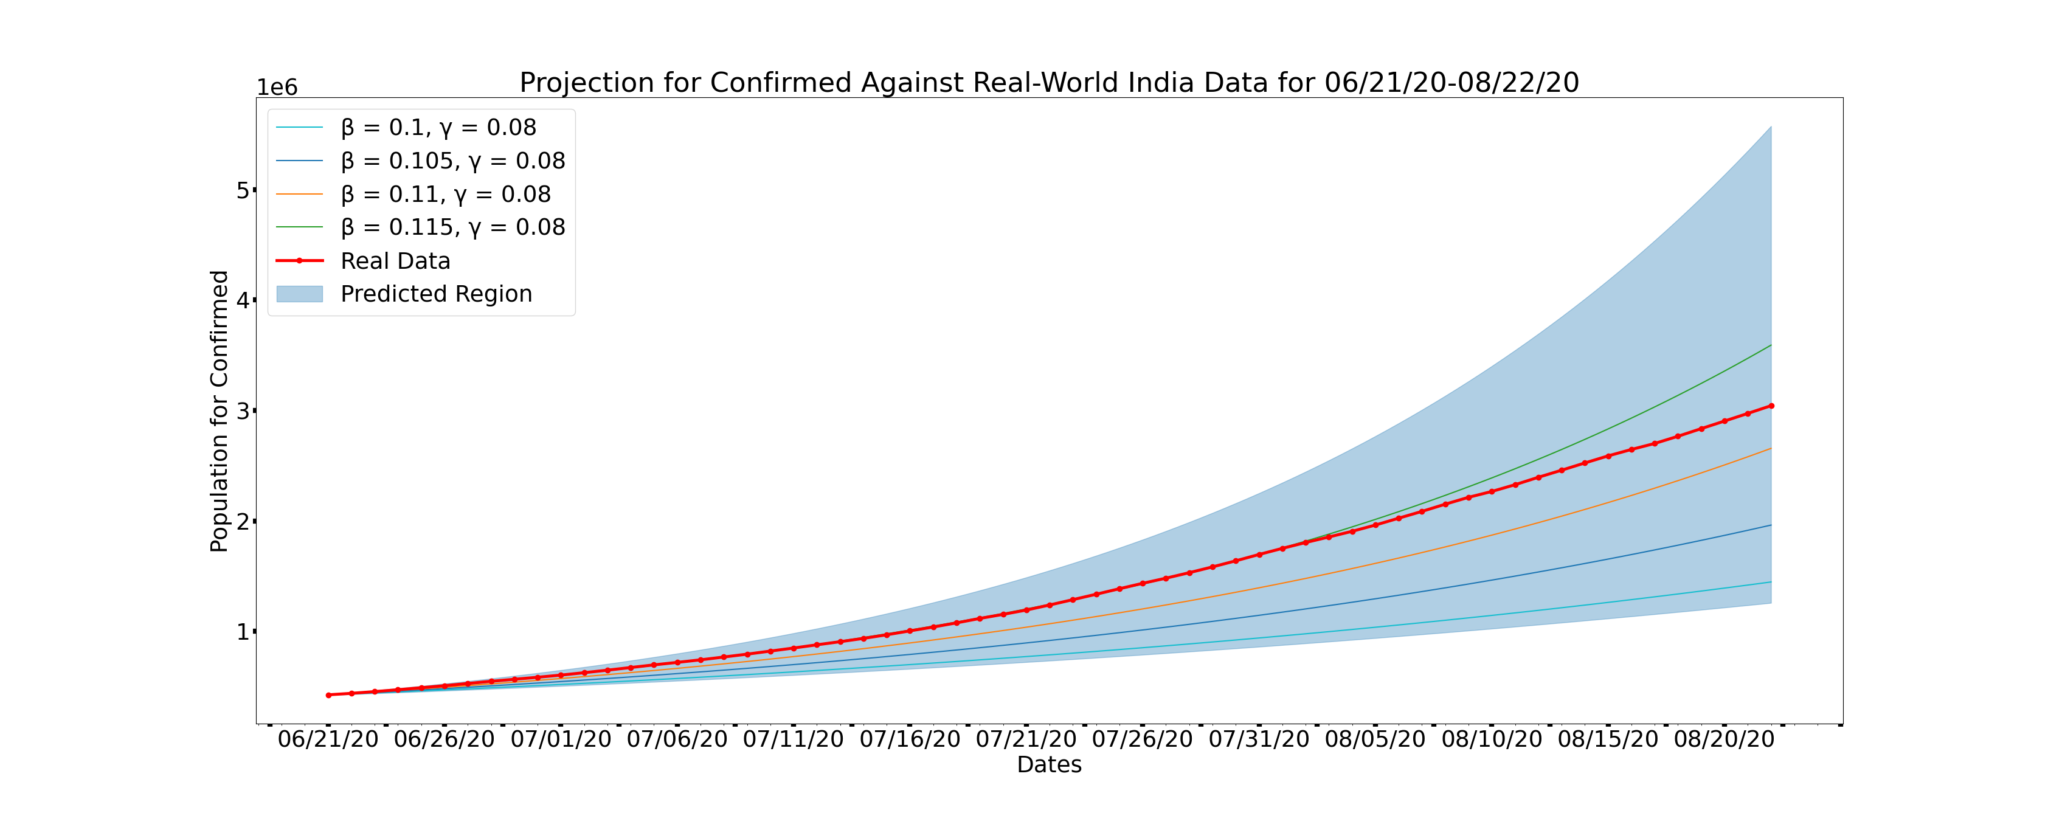
\includegraphics[width= 0.9\textwidth]{figures/IndianRecoveredPlotJun21toAug22-2-2048x813.png}
  }

  \subfloat[Confirmed population from 08/22/20-10/01/20]{
    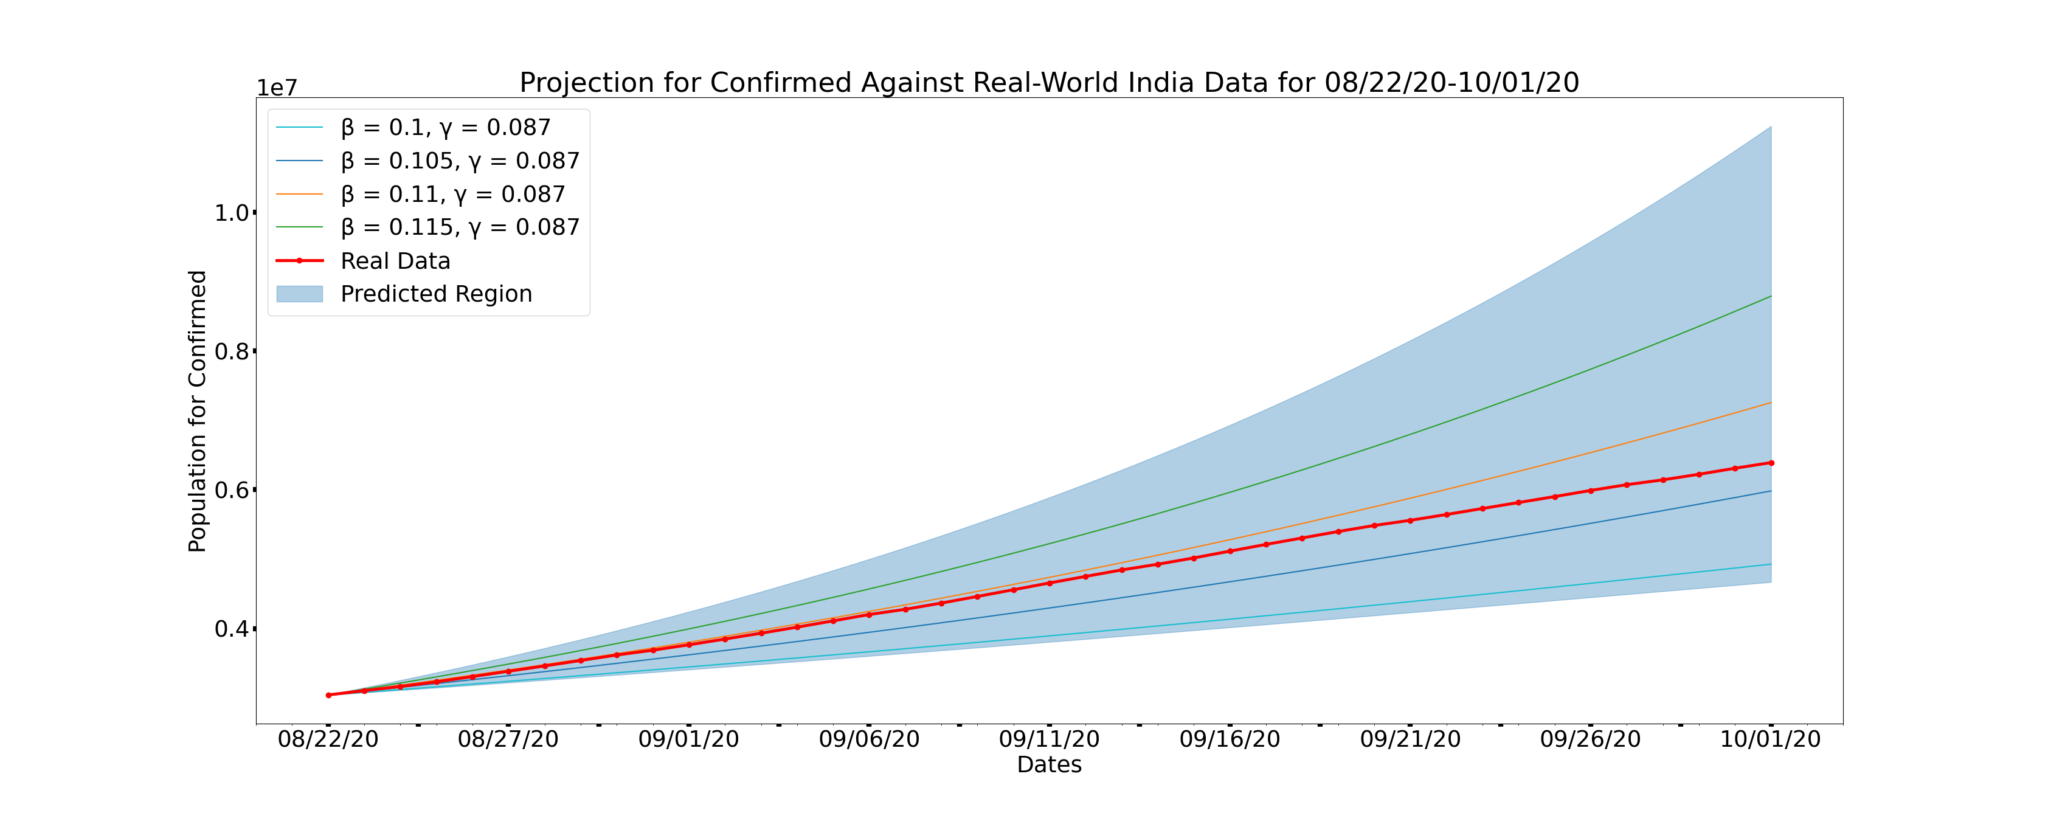
\includegraphics[width= 0.9\textwidth]{figures/IndianRecoveredPlotAug22toOct01-2-2048x813.png}
  }
\caption{Reachable Sets for India's COVID19 Confirmed Population for the period 06/21/20-10/01/20}
\label{fig:covid_plots}
\end{figure}



%-----------------------------------------------------------------------------------------------------------------------------------------------------------------
\begin{table}
%\hspace{-5em}
  \centering
\begin{tabular}{|p{1.5cm}|c|p{1.7cm}|c|c|p{5cm}|}
\hline
Model & Dimension & Parameters & \# steps & $\Delta$ & \hspace{1.5cm}Initial Box \\
\hline
Vanderpol & 2 & \quad \quad \; - & 70 steps & 0.08 & $x \in [0,0.1], y \in [1.99,2]$ \\
\hline
Jet Engine& 2 & \quad \quad \; - & 100 steps & 0.2 & $x \in [0.8,1.2], y \in [0,8,1.2]$ \\
\hline
Neuron \cite{fitzhugh1961impulses}& 2 & \quad \quad \; - & 200 steps & 0.2 & $x \in [0.9,1.1], y \in [2.4,2.6]$ \\
\hline
SIR& 3 & $\beta=0.05$ \newline $\gamma=0.34$ & 150 steps & 0.1 & $s \in [0.79,0.8], i \in [0.19,0.2], r = 0$ \\
\hline
Coupled \newline Vanderpol & 4 & \quad \quad \; - & 40 steps & 0.08 & $x1 \in [1.25, 2.25], y1 \in [1.25, 2.25]$ \newline $x2 \in [1.25, 2.25], y2 \in [1.25, 2.25]$ \\
\hline
COVID & 7 & $\beta=0.05$ \newline $\gamma=0.0$ \newline $\eta=0.02$ & 200 steps & 0.08 & \quad \quad \quad \; \; Stated Below\\
\hline
\end{tabular}
\caption{Benchmark models and relevant information}
\label{tab:modeldyns}
\end{table}
%-----------------------------------------------------------------------------------------------------------------------------------------------------------------
\section{Comparison of Template Generation Techniques}
\label{sec:compare}
%-----------------------------------------------------------------------------------------------------------------------------------------------------------------


\subsection{Accuracy of Dynamic Strategies}
\label{sec:dynamic_accuracy}
The results of testing our dynamic strategies against static ones are summarized in Table~\ref{tab:voltable}. For models previously defined in Sapo, we set the static parallelotopes to be exactly those found in Sapo.
If a model is not implemented in Sapo, we simply use the static parallelotopes defined in a model of equal dimension. To address the unavailability of a four-dimensional model implemented in Sapo, we sampled random subsets of five static non-axis-aligned parallelotopes and chose the flowpipe with smallest volume.
%
% As justifiction for this scheme, we wish to remark the time required in testing all possible subsets of diagonal parallelotopes.
%
A cursory analysis shows that the number of possible templates with diagonal directions grows with $O(n^n)$ with the number of dimensions and hence an exhaustive search on optimal template directions is infeasible.

% are $2{n \choose 2}$ diagonal directions for an $n$-dimensional system, giving a total of $n + 2 {n \choose 2}$ axis-aligned and diagonal directions. Thus, there are ${n + 2 {n \choose 2} \choose n} = {n^2 \choose n}$ possible diagonal parallelotopes for an $n$-dimensional system. This explosive growth in search space size compelled us to proceed by sampling the search space instead.

From our experiments, we conclude there is no universal optimal ratio between the number of dynamic parallelotopes defined by PCA and Linear Approxiation directions which perform well on all benchmarks. In Figure \ref{fig:PCALinAppRatio}, we demonstrate two cases where varying the ratio imparts differing effects. Observe that using parallelotopes defined by linear approximation directions is more effective than those defined by PCA directions in the Vanderpol model whereas the Neuron model shows the opposite trend.

\begin{table}[h!]
\hspace{1em}
\begin{subtable}[h]{0.45\textwidth}
     \centering
     \begin{tabular}{|c|c|}
     \hline
     Strategy & Total  Volume \\
     \hline\
     5 LinApp & 0.227911 \\
     \hline
     1 PCA, 4 LinApp& 0.225917 \\
     \hline
     2 PCA, 3 LinApp & 0.195573 \\
     \hline
     {\bf 3 PCA, 2 LinApp} & {\bf 0.188873} \\
     \hline
     4 PCA, 1 LinApp & 1.227753\\
     \hline
     5 PCA & 1.509897 \\
     \hline
     5 Static Diagonal(Sapo) & 2.863307  \\
     \hline
    \end{tabular}
    \caption{Vanderpol}
    \label{tab:vdpvol}
 \end{subtable}\hspace{1em}
 \begin{subtable}[h]{0.45\textwidth}
      \centering
      \begin{tabular}{|c|c|}
      \hline
      Strategy & Total  Volume \\
      \hline
      5 LinApp & 58199.62 \\
      \hline
      1 PCA, 4 LinApp & 31486.16 \\
      \hline
      {\bf 2 PCA, 3 LinApp} & {\bf 5204.09}\\
      \hline
      3 PCA, 2 LinApp & 6681.76 \\
      \hline
      4 PCA, 1 LinApp& 50505.10 \\
      \hline
      5 PCA  & 84191.15 \\
      \hline
      5 Static Diagonal (Sapo) & 66182.18  \\
      \hline
     \end{tabular}
     \caption{Jet Engine}
     \label{tab:enginevol}
  \end{subtable}

  \hspace{1em}
  \begin{subtable}[h]{0.45\textwidth}
       \centering
       \begin{tabular}{|c|c|}
       \hline
       Strategy & Total  Volume \\
       \hline
       5 LinApp  & 154.078\\
       \hline
       1 PCA, 4 LinApp  & 136.089\\
       \hline
       2 PCA, 3 LinApp  & 73.420\\
       \hline
       {\bf 3 PCA , 2 LinApp } & {\bf 73.126} \\
       \hline
       4 PCA, 1 LinApp  & 76.33 \\
       \hline
       5 PCA & 83.896 \\
       \hline
       5 Static Diagonal  (Sapo) & 202.406  \\
       \hline
      \end{tabular}
      \caption{FitzHugh-Nagumo}
      \end{subtable} \hspace{1em}
      \begin{subtable}[h]{0.45\textwidth}
        \centering
        \begin{tabular}{|c|c|}
        \hline
        Strategy & Total  Volume \\
        \hline
        {\bf 2 LinApp } & {\bf 0.001423} \\
        \hline
        1 PCA, 1 LinApp & 0.106546\\

        \hline
        2 PCA  & 0.117347\\
        \hline
        2 Static Diagonal (Sapo) & 0.020894\\
        \hline
       \end{tabular}
       \caption{SIR}
       \label{tab:sirvol}
    \end{subtable}

    \hspace{1em}
    \begin{subtable}[h]{0.45\textwidth}
         \centering
         \begin{tabular}{|c|c|}
         \hline
         Strategy & Total  Volume \\
         \hline
         5 LinApp & 5.5171 \\
         \hline
         {\bf 1 PCA, 4 LinApp } & {\bf 5.2536} \\
         \hline
         2 PCA, 3 LinApp  & 5.6670\\
         \hline
         3 PCA, 2 LinApp  & 5.5824\\
         \hline
         4 PCA, 1 LinApp  & 312.2108 \\
         \hline
         5 PCA  & 388.0513 \\
         \hline
         5 Static Diagonal (Best) & 3023.4463  \\
         \hline
        \end{tabular}
        \caption{Coupled Vanderpol}
        \label{tab:sirvol}
     \end{subtable}\hspace{1 em}
    \begin{subtable}[h]{0.45\textwidth}
         \centering
         \begin{tabular}{|c|c|}
         \hline
         Strategy & Total  Volume \\
         \hline
         3 LinApp & $2.95582227 * 10^{-10}$ \\
         \hline
         {\bf 1 PCA, 2 LinApp } & {\bf $2.33007583 * 10^{-10}$}\\
         \hline
         2 PCA, 1 LinApp &$ 4.02751770 * 10^{-9}$\\
         \hline
         3 PCA & $4.02749571 * 10^{-9}$\\
         \hline
         3 Static Diagonal (Sapo) & $4.02749571 * 10^{-9}$\\
         \hline
        \end{tabular}
        \caption{COVID}
        \label{tab:covidvol}
     \end{subtable}
 \caption{Tables presenting upper bounds on the total reachable set volume by strategy. The static directions are retrieved and/or inspired from Sapo models of equal dimension for benchmarking. The best performing strategy is highlighted in bold.}
     \label{tab:voltable}
\end{table}


%\begin{figure}[h!]
\begin{subfigure}
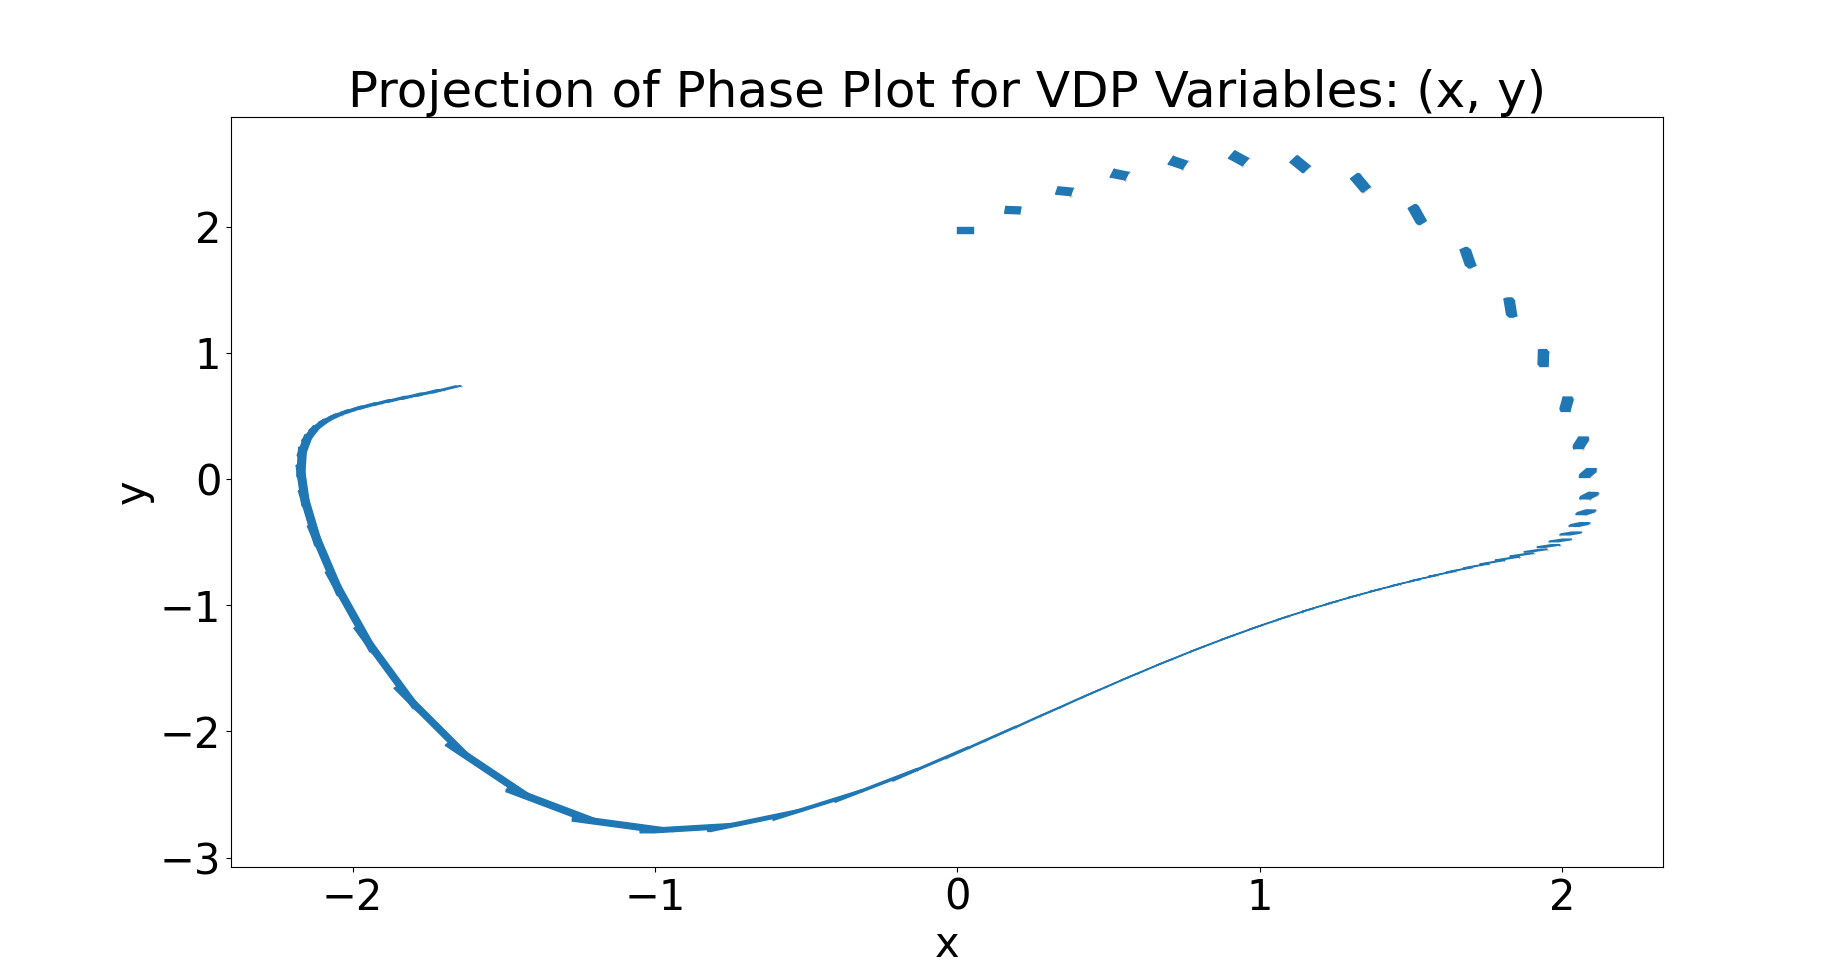
\includegraphics[width=\textwidth]{figures/PhasePlots/VDP_5Lin_.png}
\caption{5 Lin}
\end{subfigure}%
\begin{subfigure}
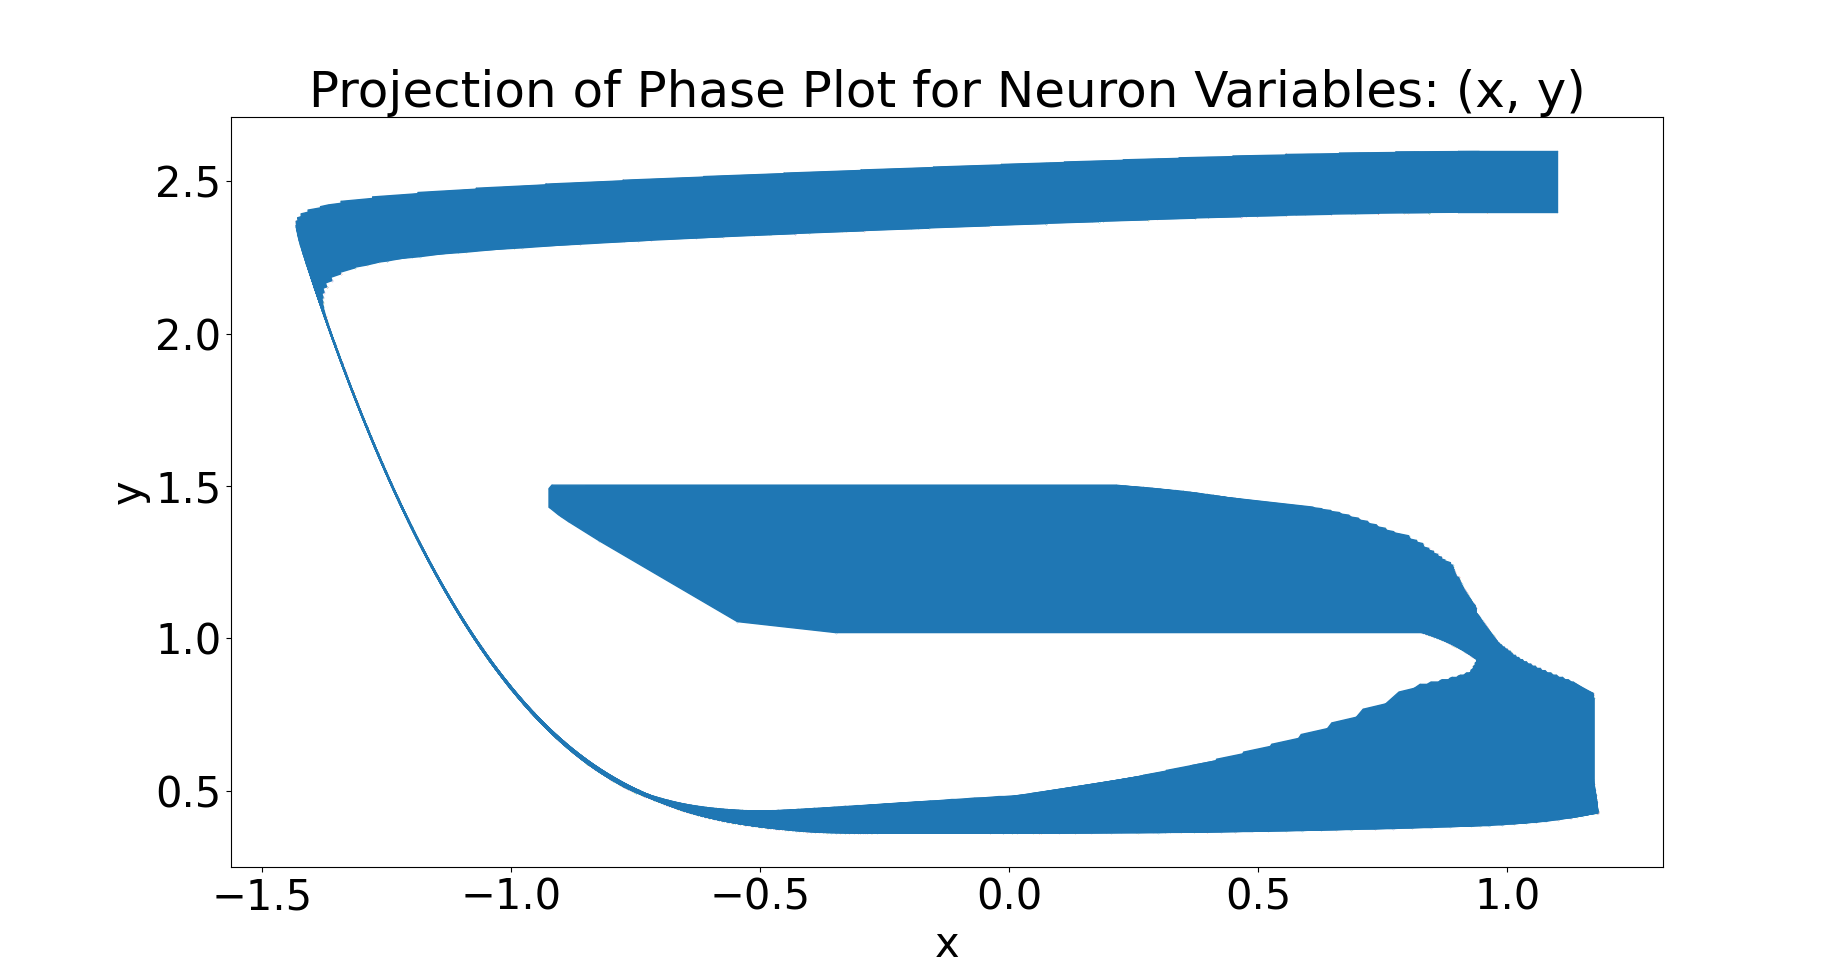
\includegraphics[width=\textwidth]{figures/PhasePlots/Neuron_1PCA5Lin_.png}
\caption{1 PCA 5 Lin}
\end{subfigure}%

\begin{subfigure}
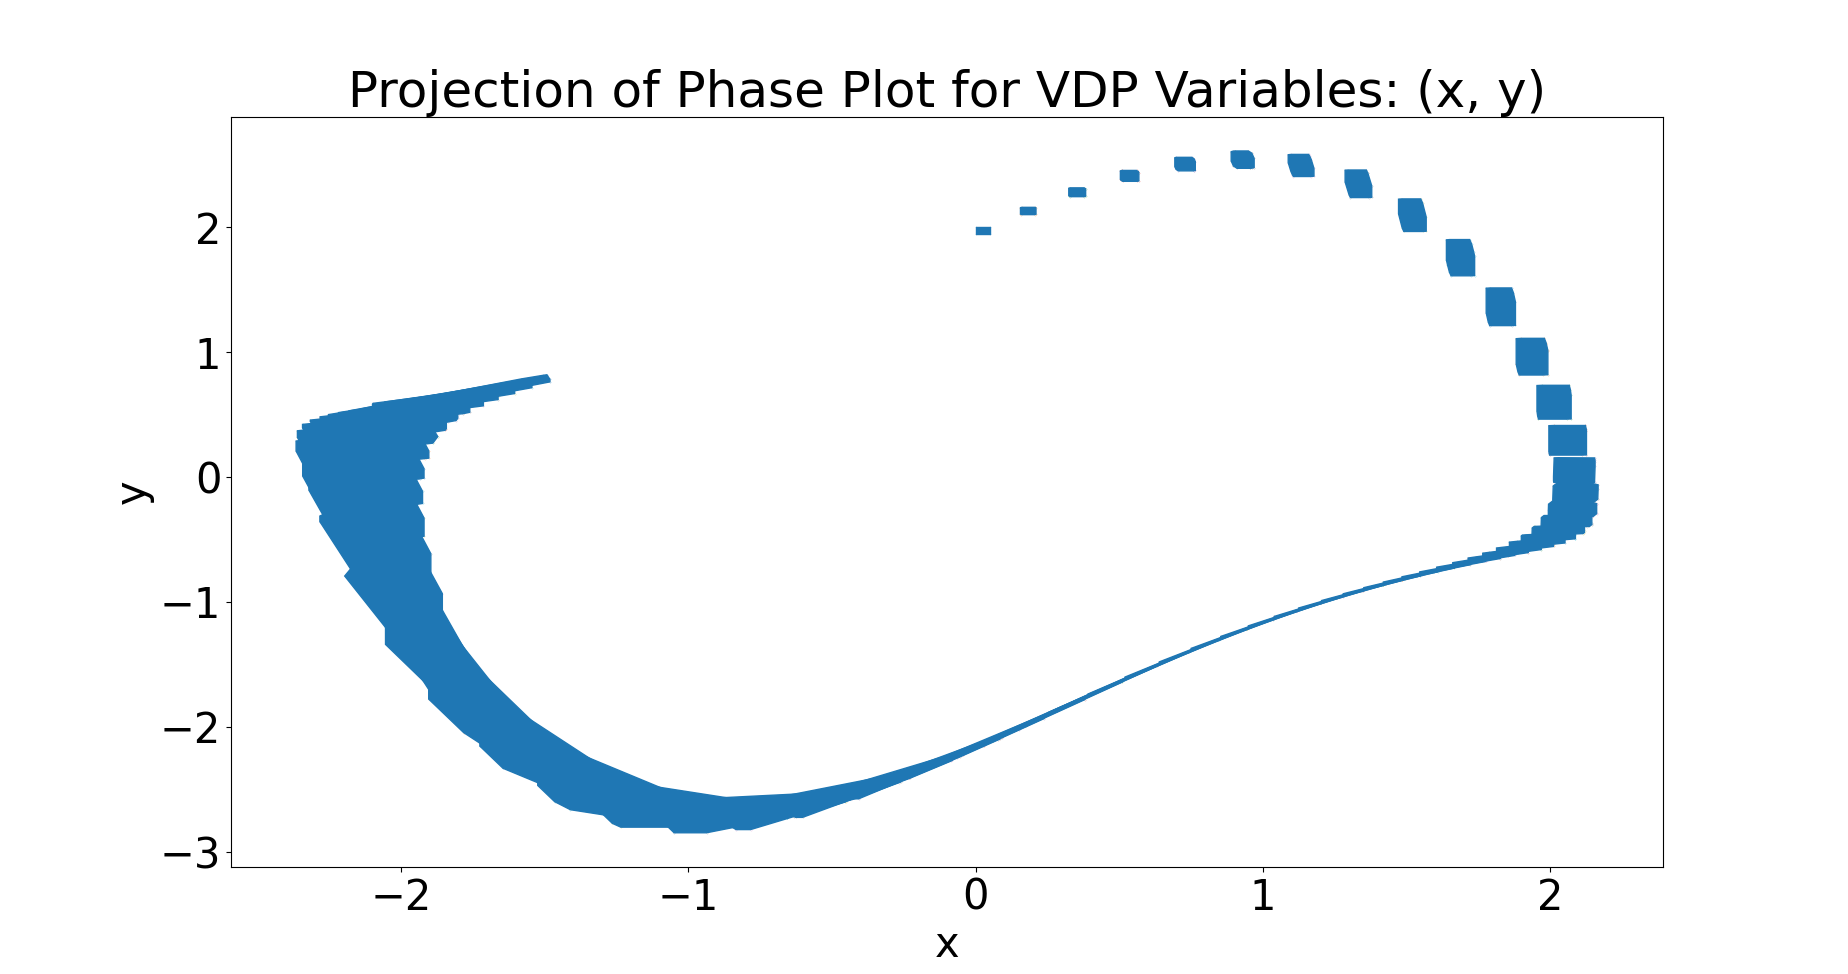
\includegraphics[width=\textwidth]{figures/PhasePlots/VDP_5PCA_.png}
\caption{5 PCA}
\end{subfigure}%
\begin{subfigure}
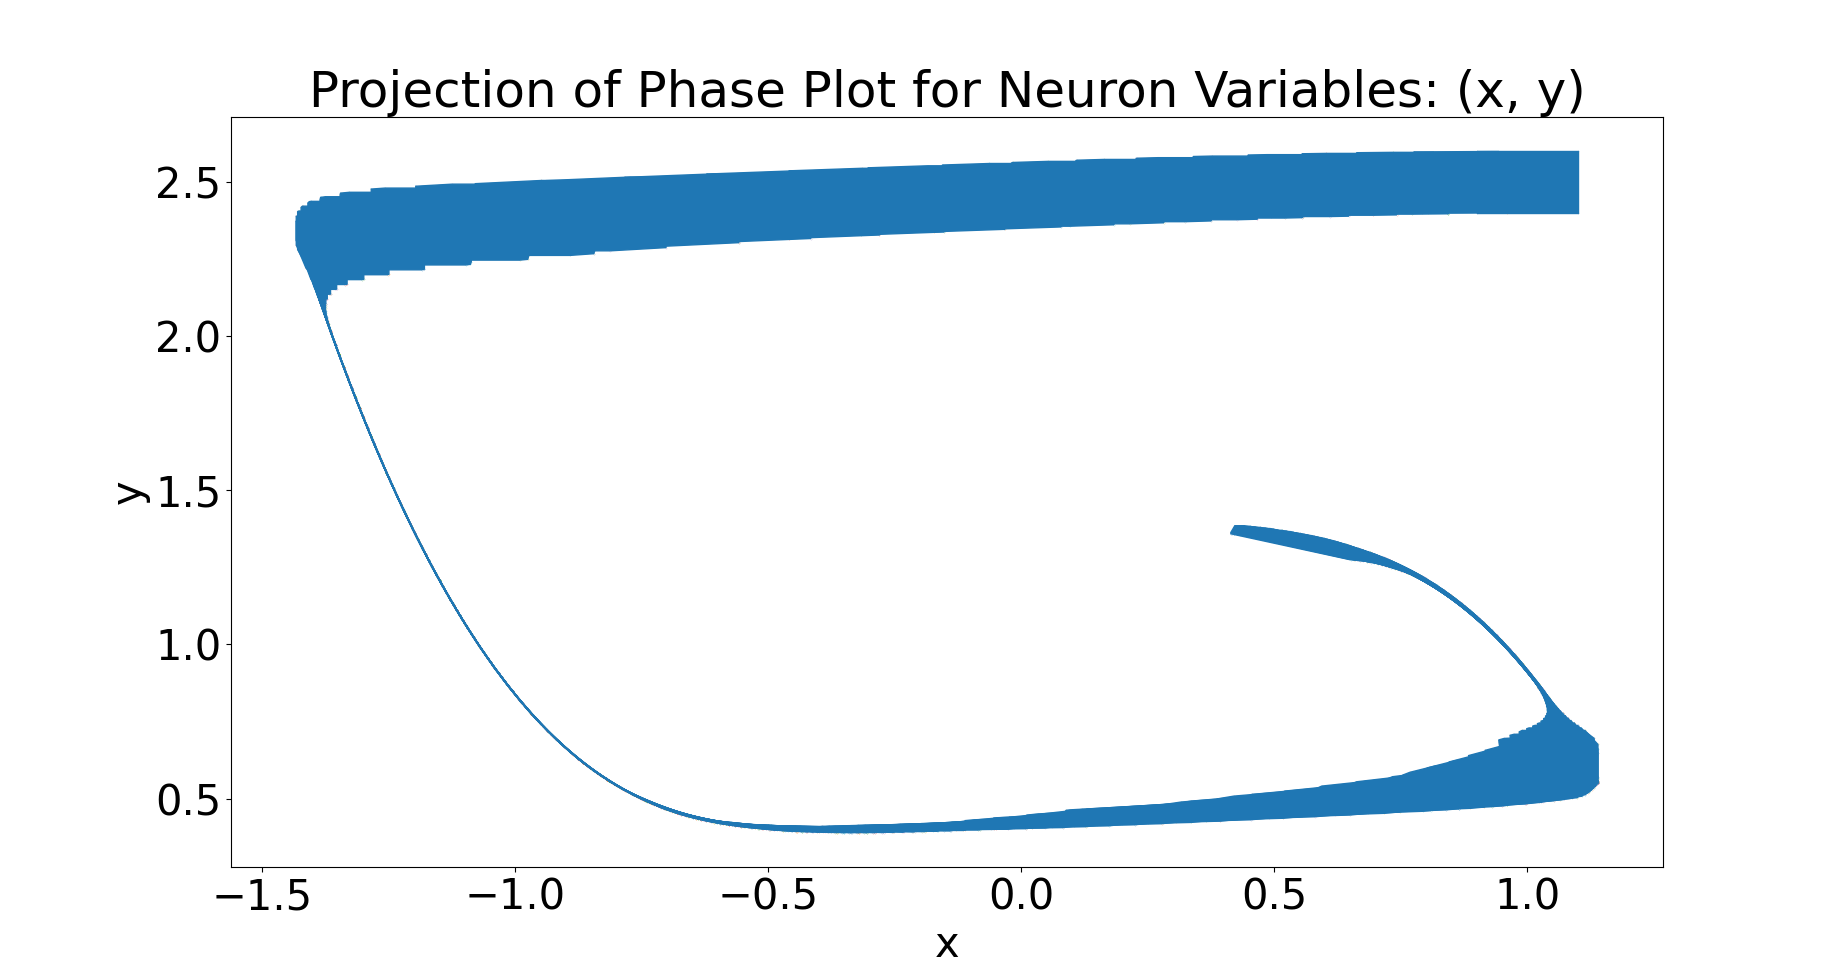
\includegraphics[width=\textwidth]{figures/PhasePlots/Neuron_5PCA1Lin_.png}
\caption{5 PCA 1 Lin}
\end{subfigure}

\begin{subfigure}
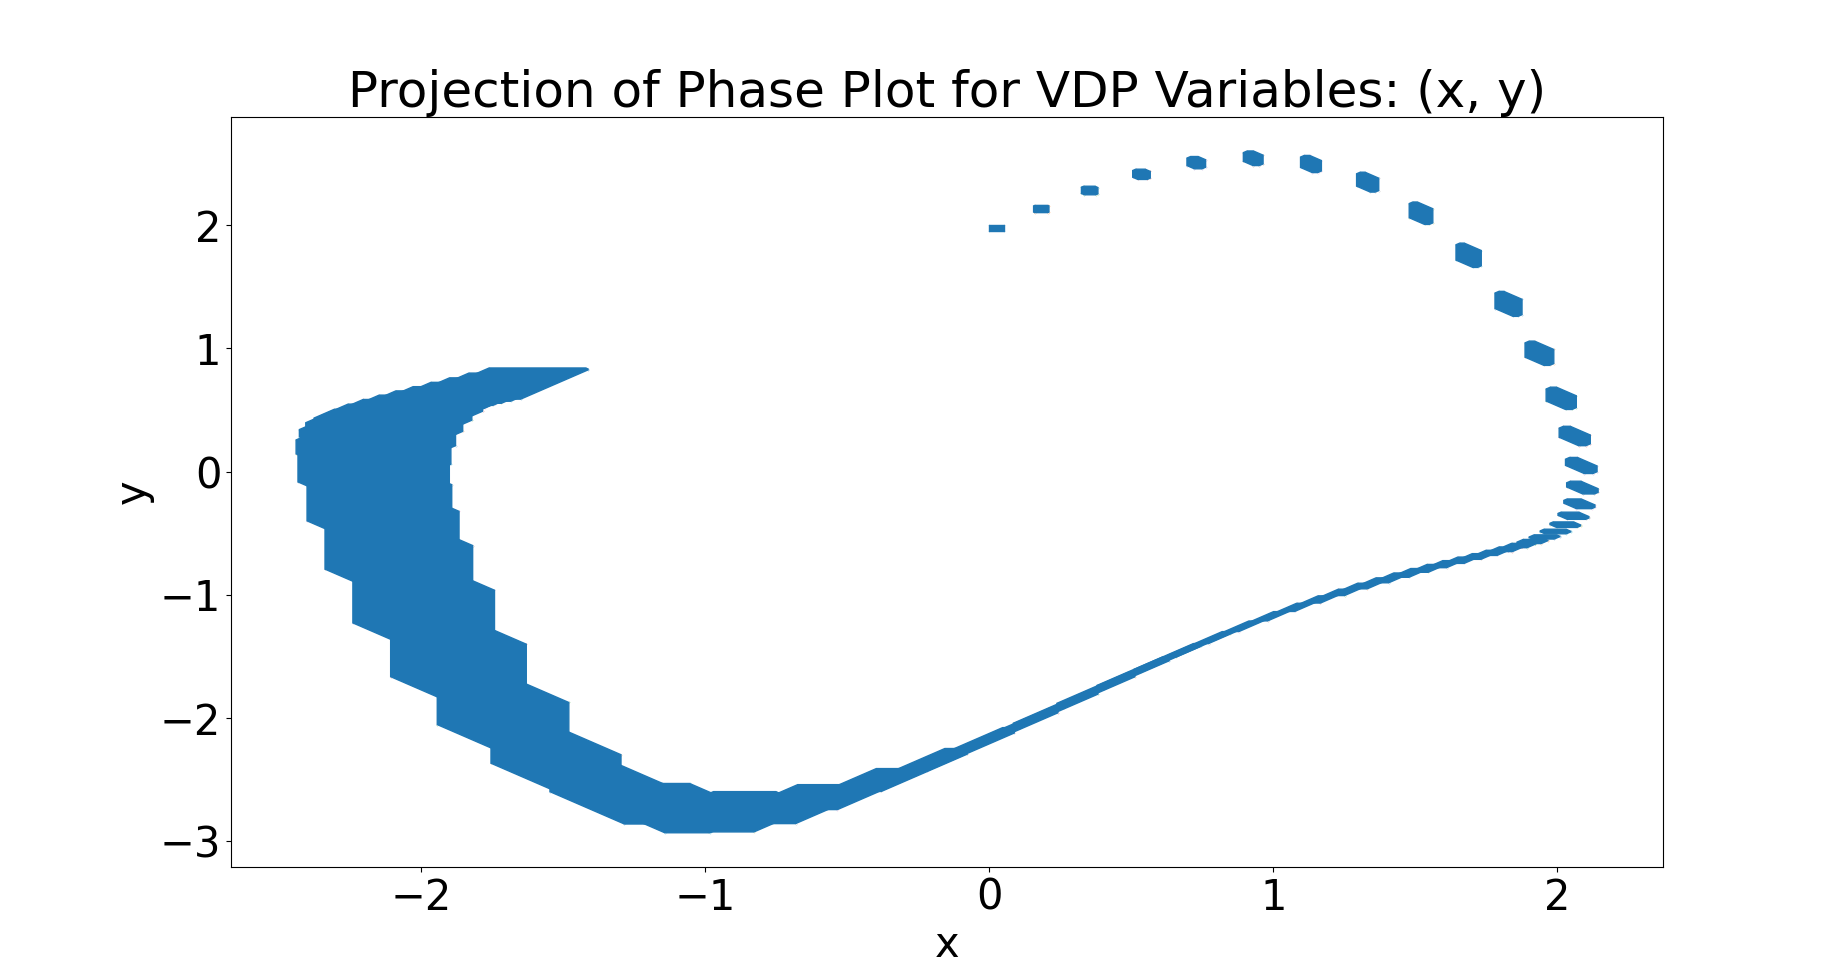
\includegraphics[width=\textwidth]{figures/PhasePlots/VDP_Sapo_.png}
\caption{Sapo}
\end{subfigure}%
\begin{subfigure}
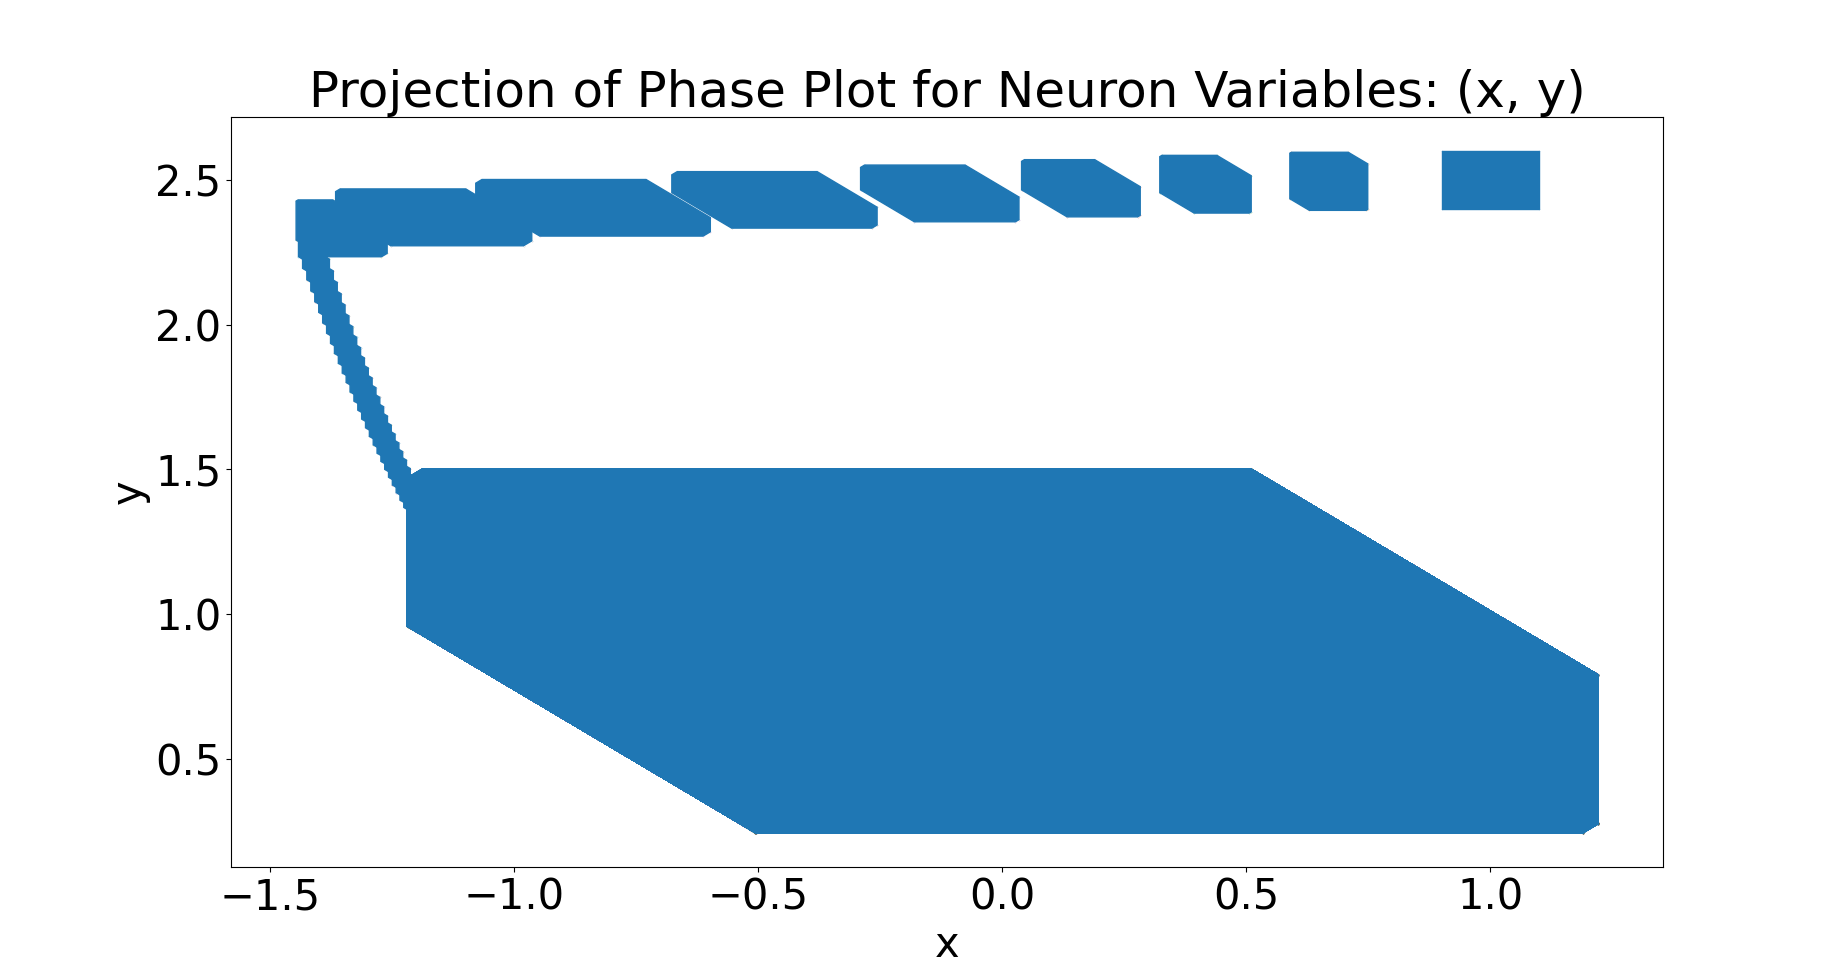
\includegraphics[width=\textwidth]{figures/PhasePlots/Neuron_Sapo_.png}
\caption{Sapo}
\end{subfigure}
\caption{Effect of varying ratio between the number of PCA and Linear Approximation parallelotopes. The Vanderpol (left) and the FitzHugh-Nagumo Neuron (right) phase plots are shown to illustrate differing effects of varying the PCA/LinApp ratio. The initial set for the Vanderpol model is set to $x \in [0,0.05], \, y \in [1.95,2]$}
\label{fig:PCALinAppRatio}
\end{figure}



%-----------------------------------------------------------------------------------------------------------------------------------------------------------------
\subsection{Performance under Increasing Initial Sets}
\label{sec:increasing_initial}

A key advantage of our dynamic strategies is the improved ability to control the wrapping error naturally arising from larger initial sets. Figure \ref{fig:InitVolReachComp} presents charts showcasing the effect of increasing initial sets on the total flowpipe volume. We vary the initial box dimensions to gradually increase the box's volume. We then plot the total flowpipe volume after running the benchmark. The same initial boxes are also used in computations using Sapo's static parallelotopes. The number of parallelotopes defined by PCA and Linear Approximation directions were chosen based on best performance as seen in Table \ref{tab:voltable}. We remark that our dynamic strategies perform better than static ones in controlling the total flowpipe volume as the initial set becomes larger. On the other hand, the performance of static parallelotopes tends to degrade rapidly as we increase the volume of the initial box.

\def \initvolwidth {0.6}
\def \initvolheight {0.5}
\def \initvolhorshift {-1.5cm}
\def \initvolvertshift {-2cm}

\begin{figure}
  \centering
  \vspace*{\initvolvertshift}
    \hspace*{\initvolhorshift}\subfloat[Vanderpol]{
    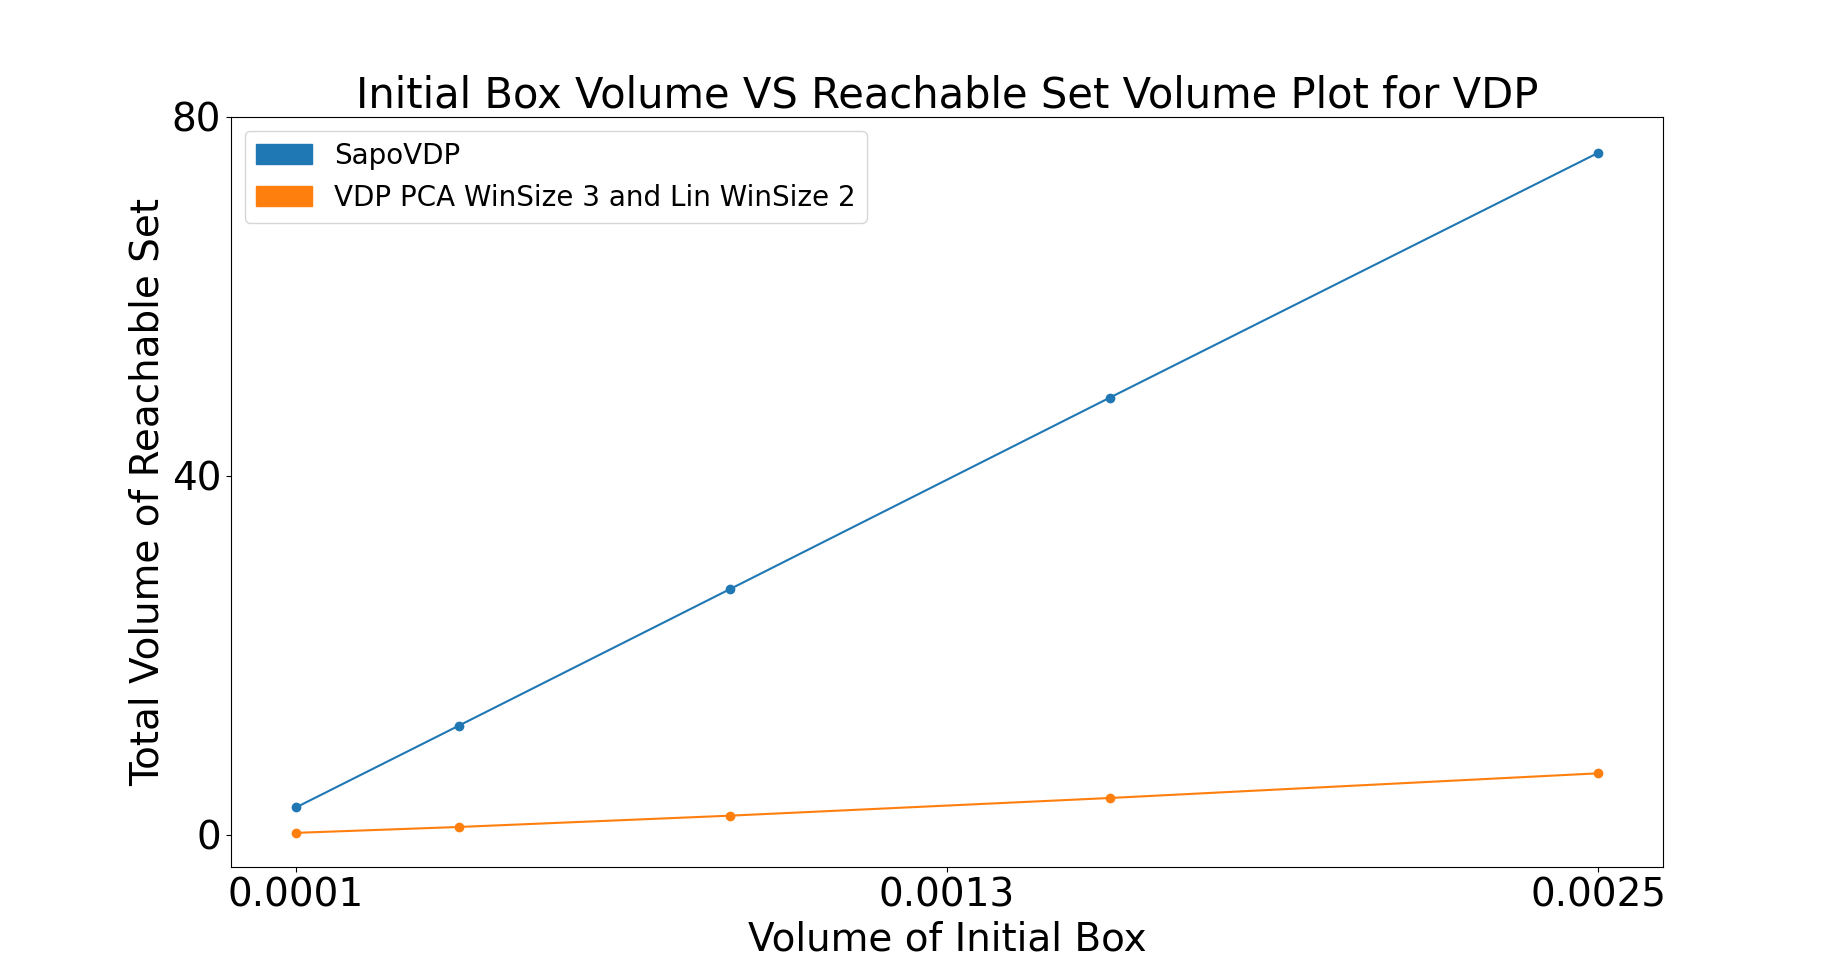
\includegraphics[width=\initvolwidth\textwidth, height=\initvolheight \textwidth]{figures/InitVolVSReachVol/VDPInitReachVol.png}
  }
  \subfloat[Jet Engine]{
  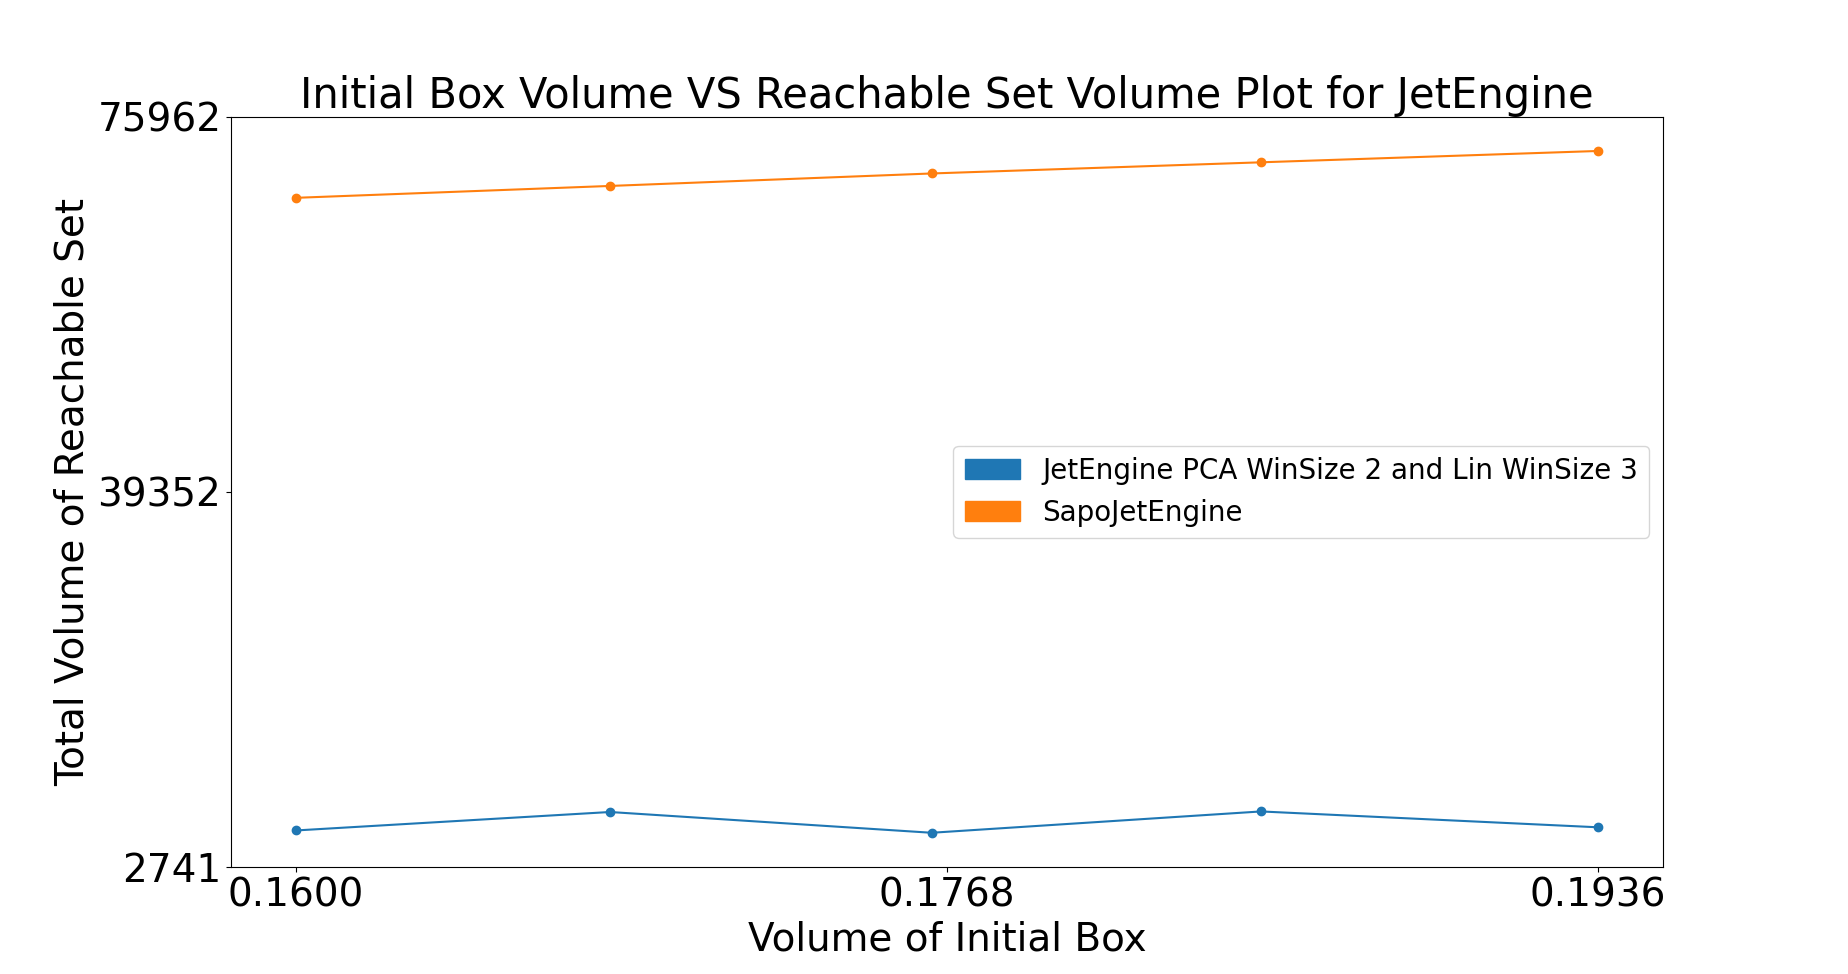
\includegraphics[width=\initvolwidth\textwidth, height=\initvolheight \textwidth]{figures/InitVolVSReachVol/JetEngineInitReachVol.png}
  }

  \hspace*{\initvolhorshift}\subfloat[Neuron]{
    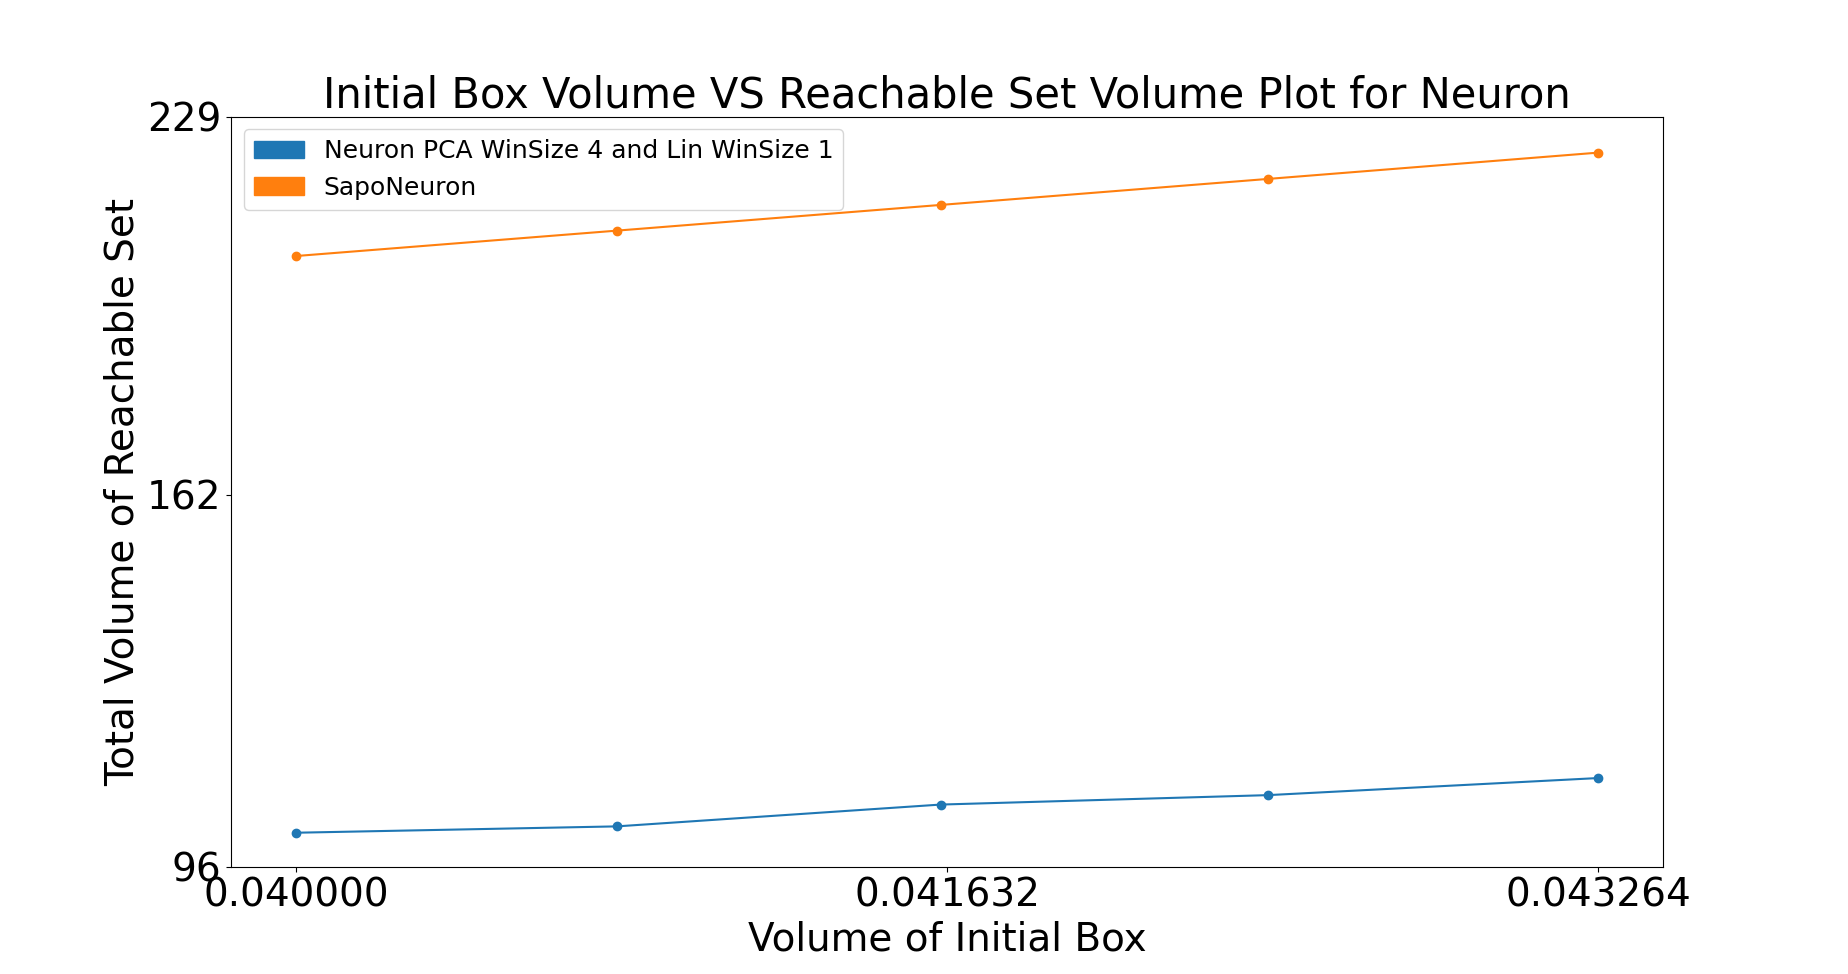
\includegraphics[width=\initvolwidth\textwidth, height=\initvolheight \textwidth]{figures/InitVolVSReachVol/NeuronInitReachVol200steps.png}
  }
  \subfloat[Coupled Vanderpol]{
  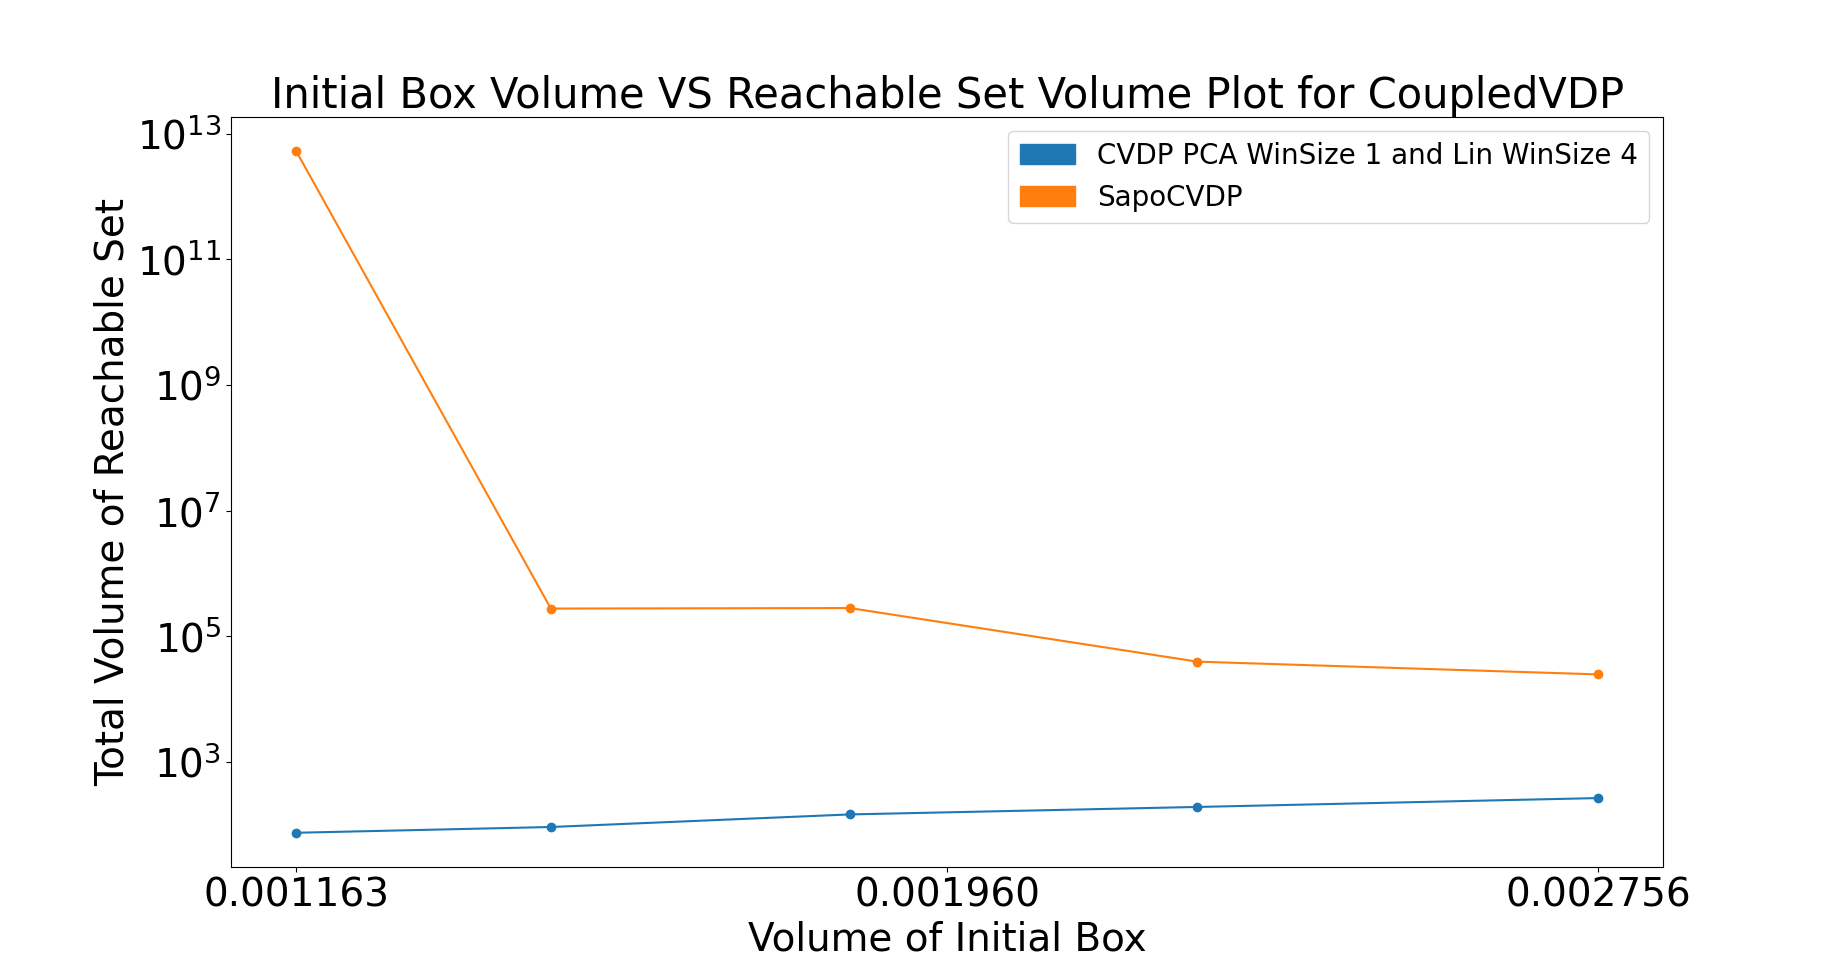
\includegraphics[width=\initvolwidth\textwidth, height=\initvolheight \textwidth]{figures/InitVolVSReachVol/CVDPInitReachVol.png}
  }

  \hspace*{\initvolhorshift}\subfloat[SIR]{
  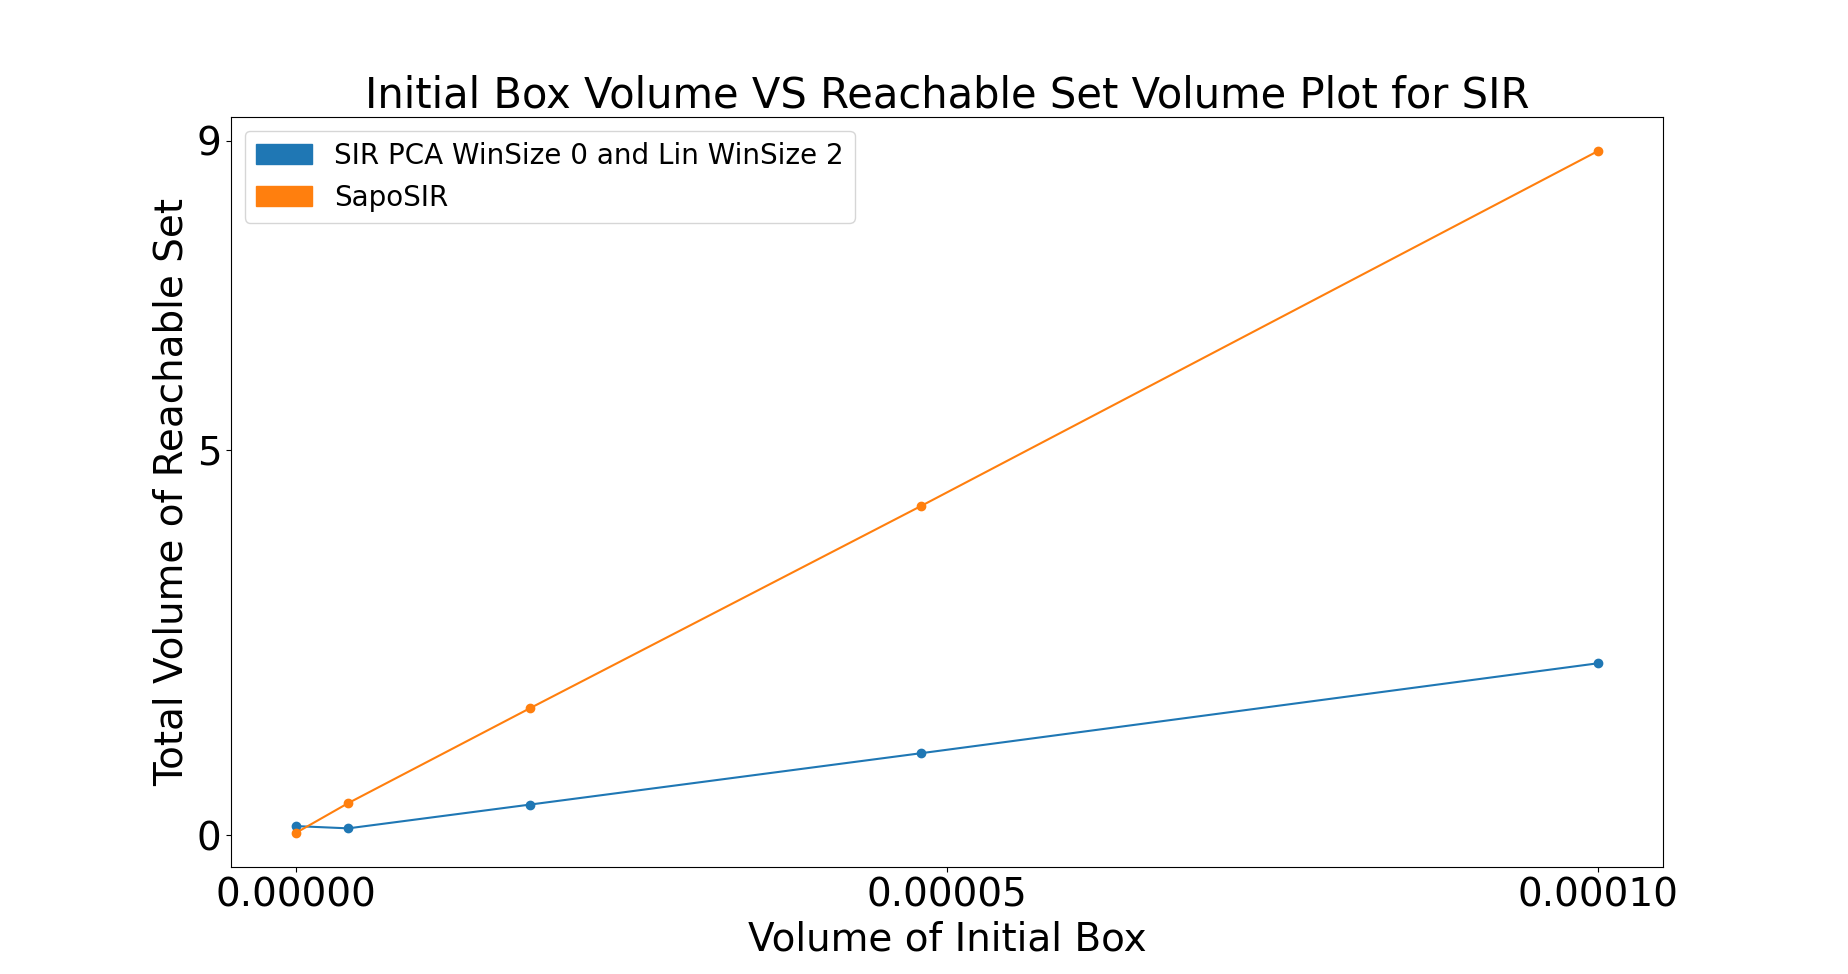
\includegraphics[width=\initvolwidth\textwidth, height=\initvolheight \textwidth]{figures/InitVolVSReachVol/SIRInitReachVol.png}
  }
  \subfloat[COVID]{
  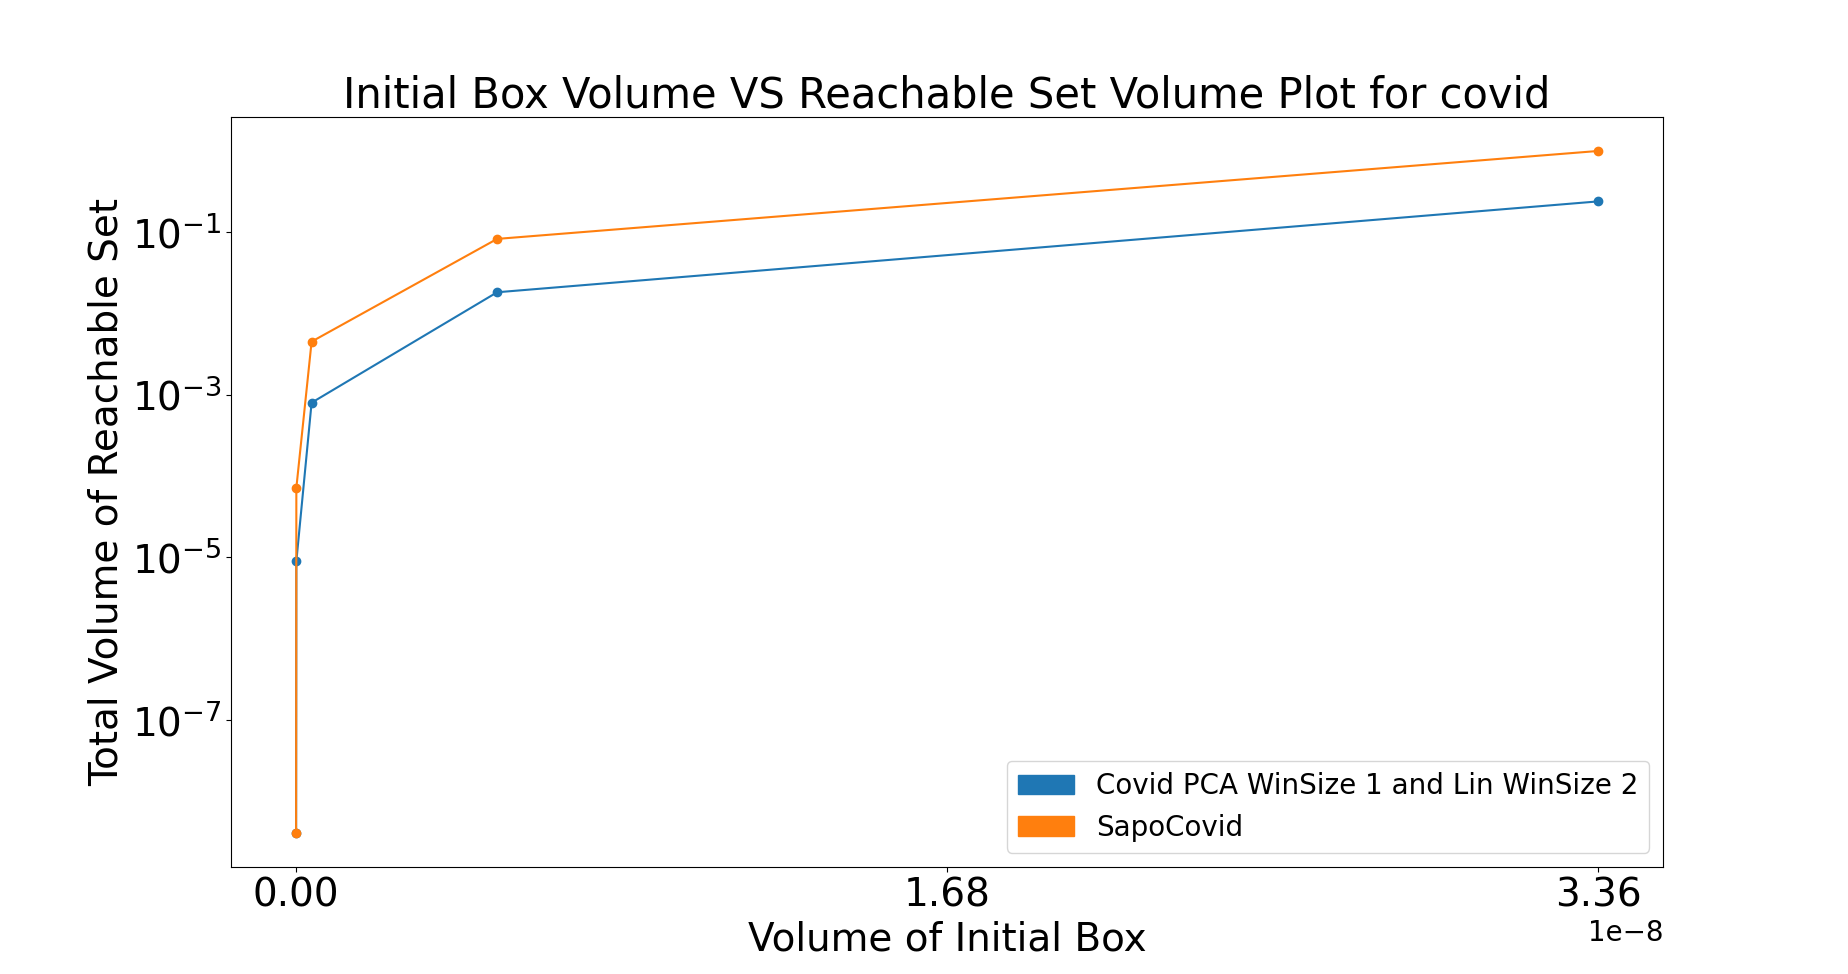
\includegraphics[width=\initvolwidth\textwidth, height=\initvolheight \textwidth]{figures/InitVolVSReachVol/CovidInitReachVol.png}
  }

  \caption{Comparison between the performance of diagonal static parallelotope bundles and that of the best performing dynamic parallelotope bundles as the volume of the initial set grows.}
  \label{fig:InitVolReachComp}
\end{figure}



\subsection{Performance against Random Static Templates}
\label{sec:random_static}

We additionally benchmark our dynamic strategies against static random parallelotope bundles. We sample such parallelotopes in $n$ dimensions by first sampling a set of $n$ directions uniformly on the surface of the unit $(n-1)$-sphere, then defining our parallelotope using these sampled directions. We sample twenty of these parallelotopes for each trial and average the total flowpipe volumes. As shown in Figure \ref{fig:RanStaticStratComp}, our best-performing dynamic strategies consistently outperform static random strategies for all tested benchmarks.

\def \randvolwidth {0.6}
\def \randvolheight {0.5}
\def \randvolhorshift {-1.5cm}
\def \randvolvertshift {-2cm}

\begin{figure}
  \centering
  \vspace*{\randvolvertshift}
    \hspace*{\randvolhorshift}\subfloat[Vanderpol]{
    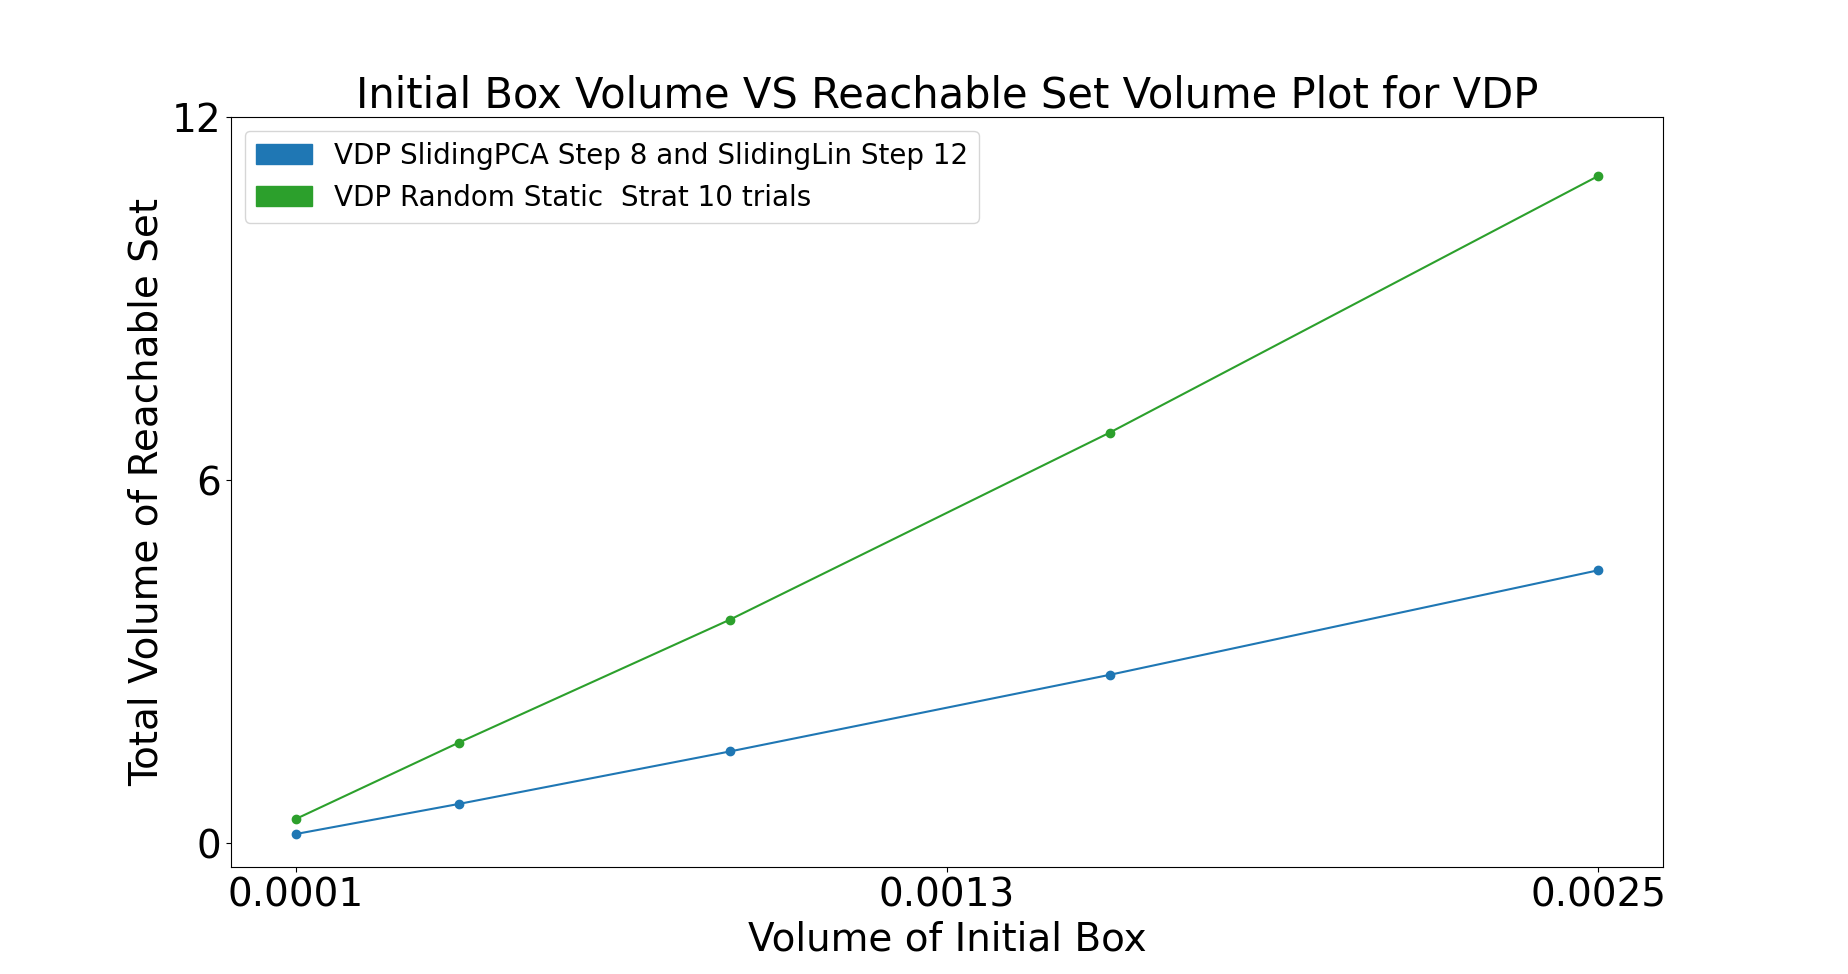
\includegraphics[width=\initvolwidth\textwidth, height=\initvolheight \textwidth]{figures/InitVolVSReachVol/VDPInitReachVolRanStrat.png}
  }
  \subfloat[Jet Engine]{
  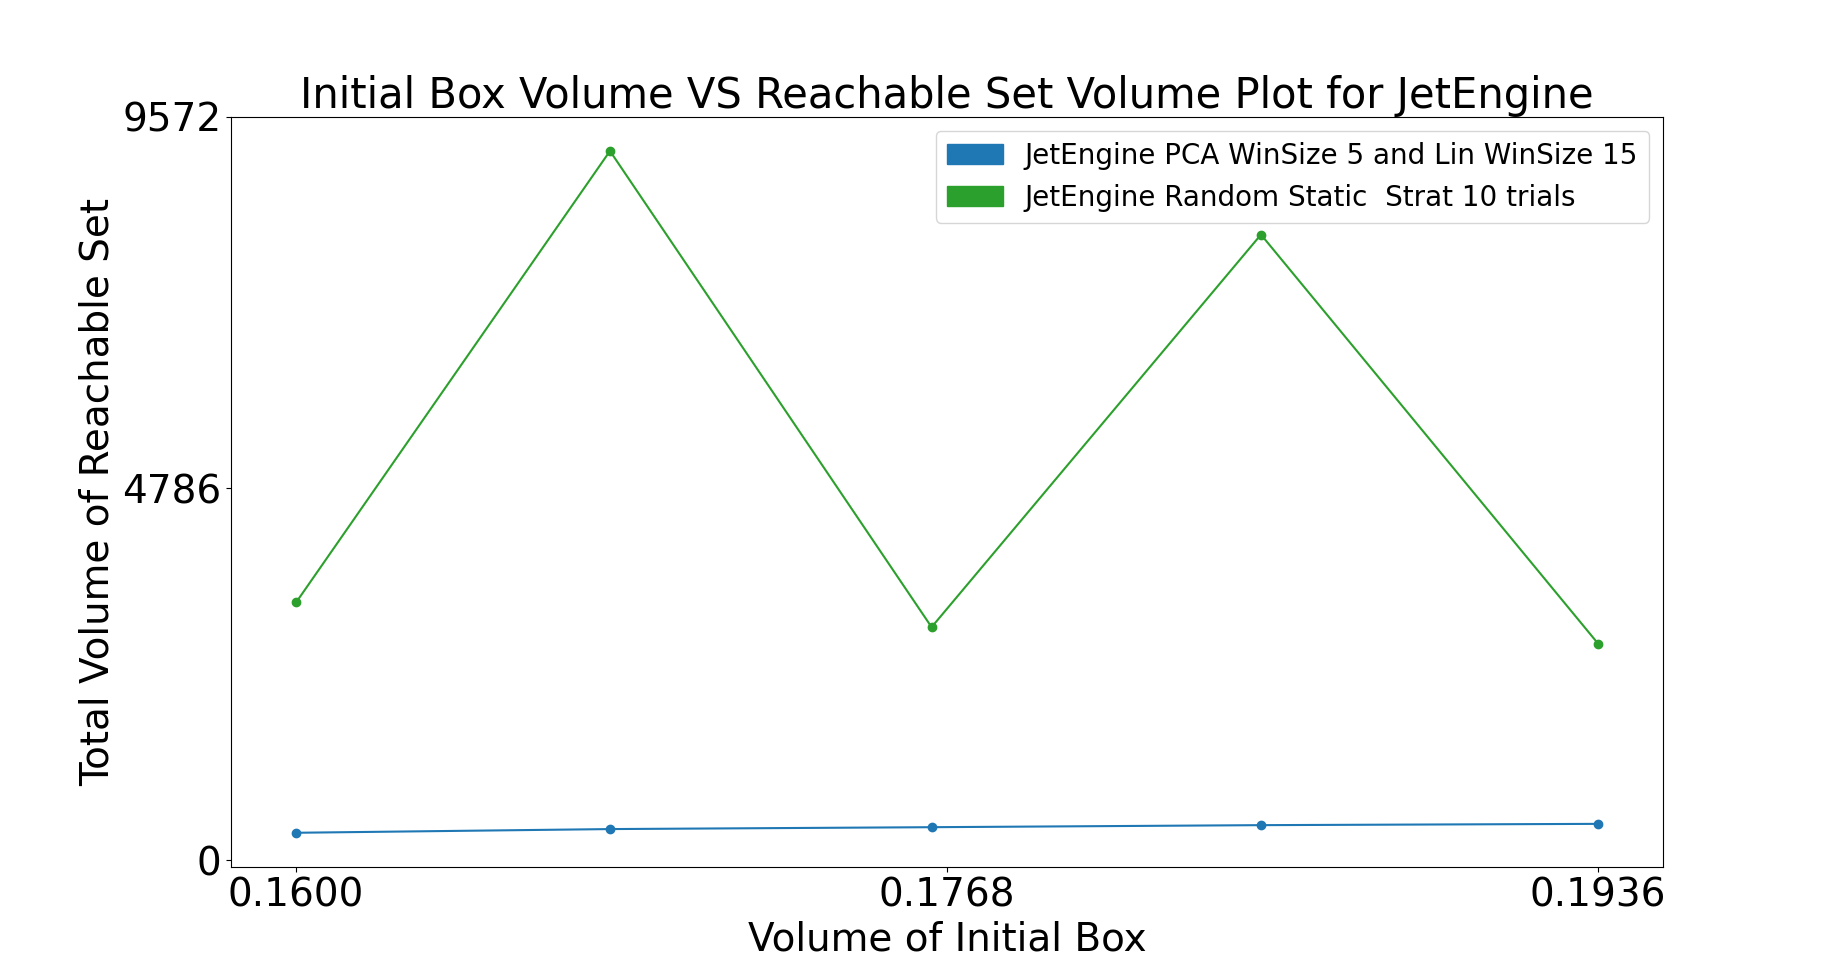
\includegraphics[width=\initvolwidth\textwidth, height=\initvolheight \textwidth]{figures/InitVolVSReachVol/JetEngineInitReachVolRanStrat.png}
  }

  \hspace*{\randvolhorshift}\subfloat[Neuron]{
    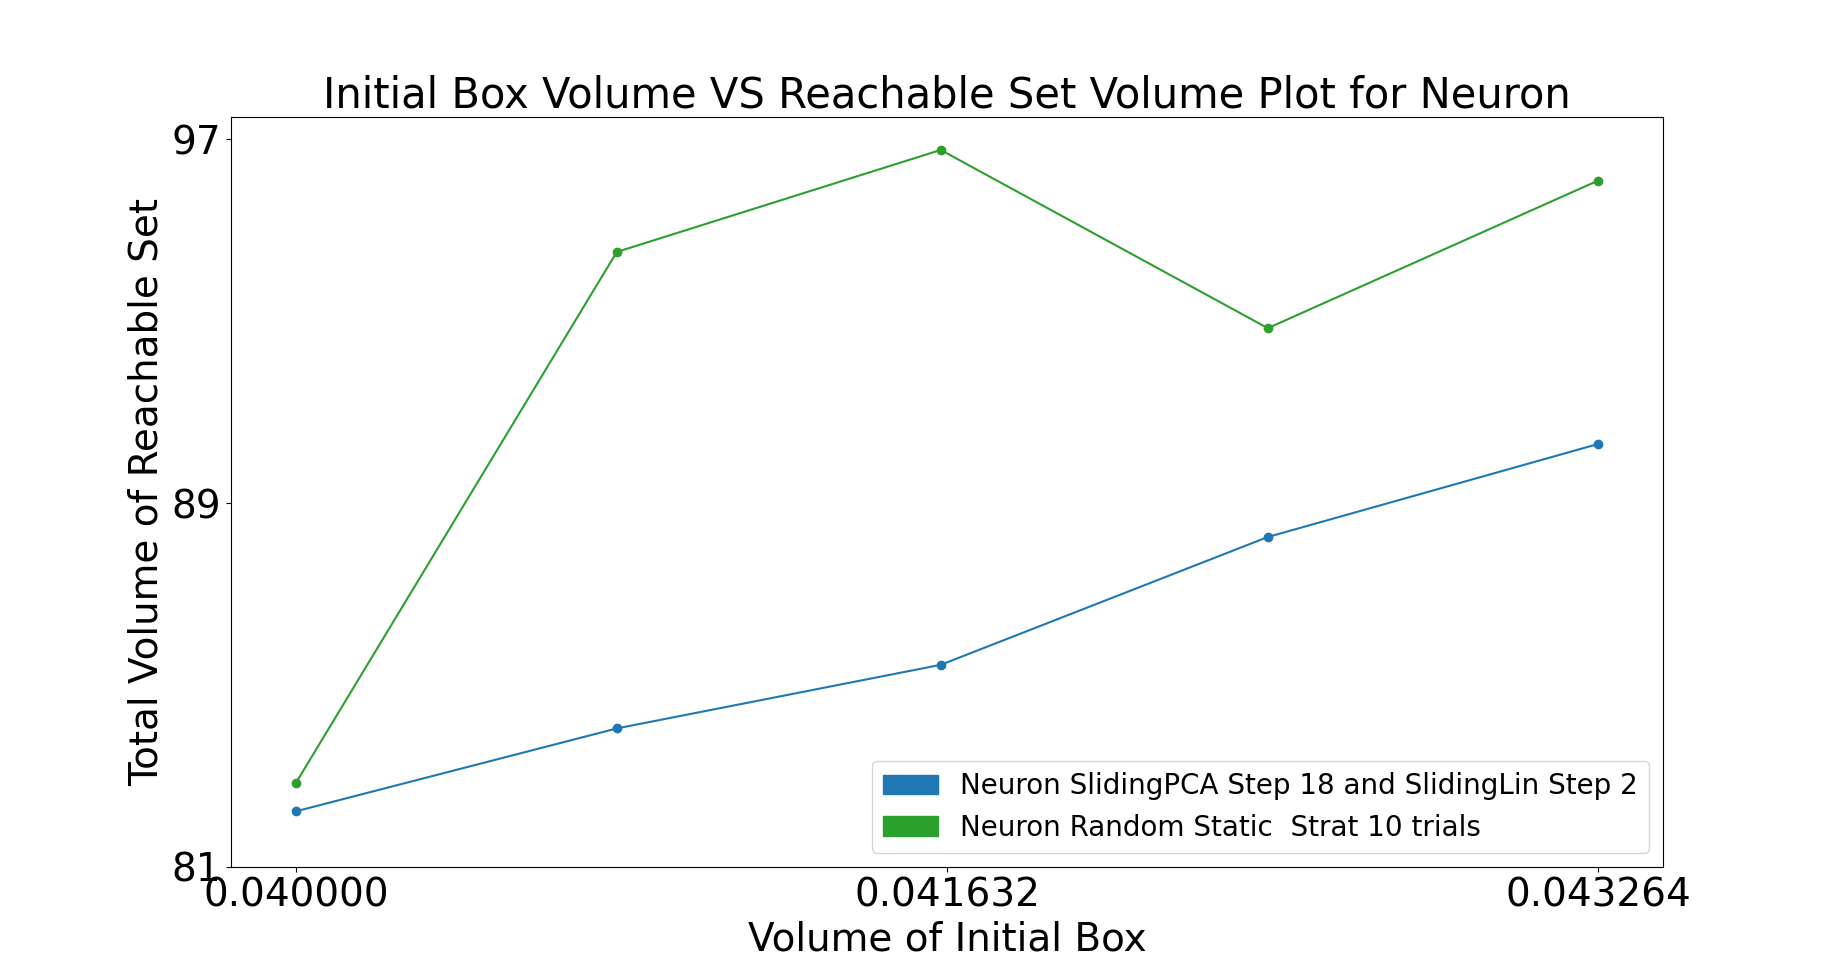
\includegraphics[width=\initvolwidth\textwidth, height=\initvolheight \textwidth]{figures/InitVolVSReachVol/NeuronInitReachVolRanStrat.png}
  }
  \subfloat[Coupled Vanderpol]{
  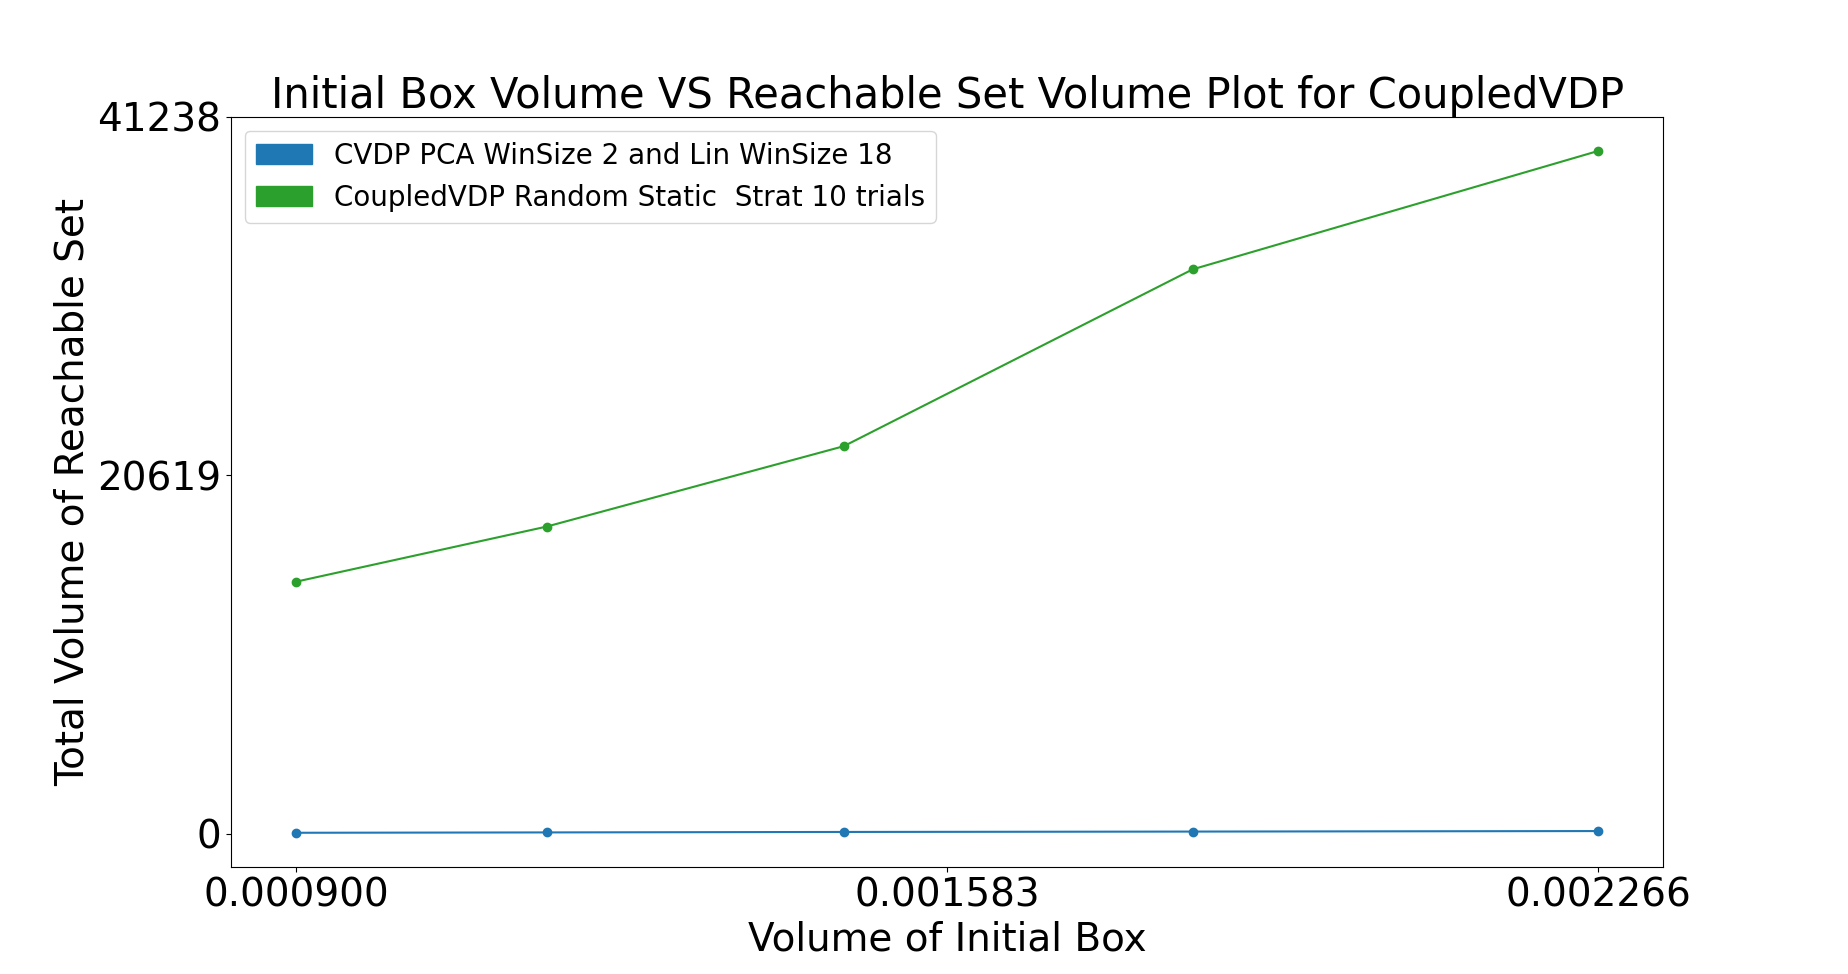
\includegraphics[width=\initvolwidth\textwidth, height=\initvolheight \textwidth]{figures/InitVolVSReachVol/CVDPInitReachVolRanStrat.png}
  }

  \hspace*{\randvolhorshift}\subfloat[SIR]{
  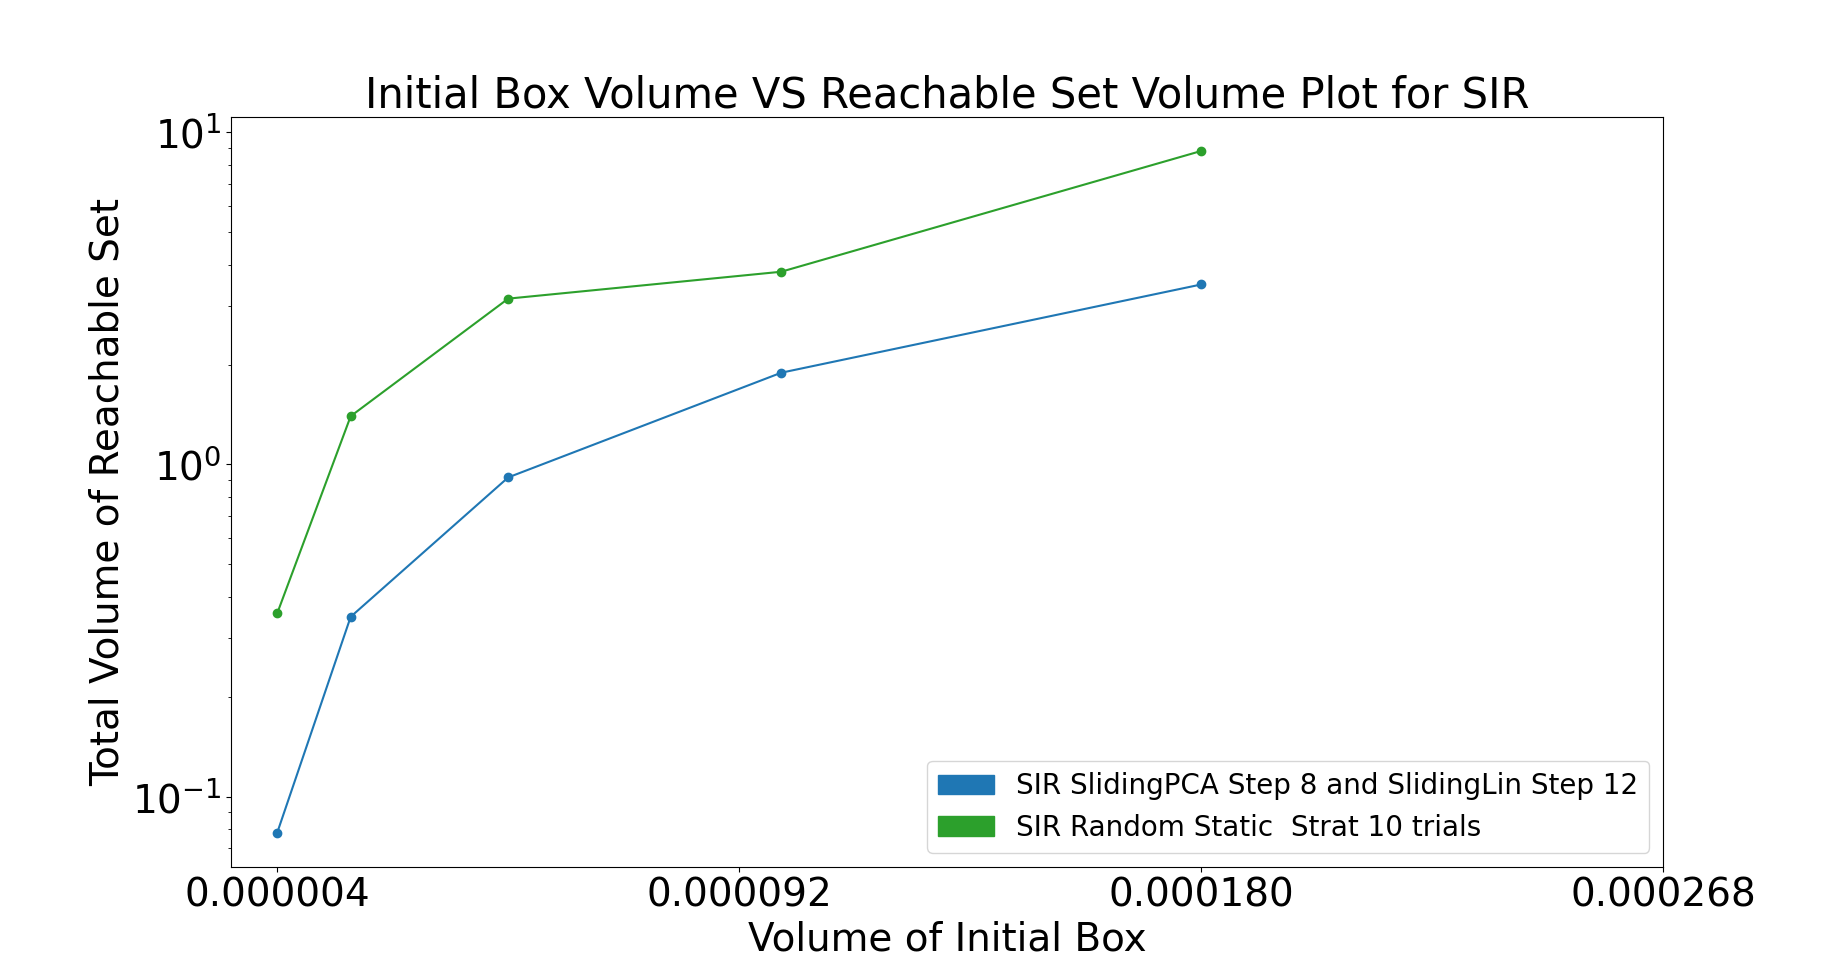
\includegraphics[width=\initvolwidth\textwidth, height=\initvolheight \textwidth]{figures/InitVolVSReachVol/SIRInitReachVolRanStrat.png}
  }
  \subfloat[COVID]{
  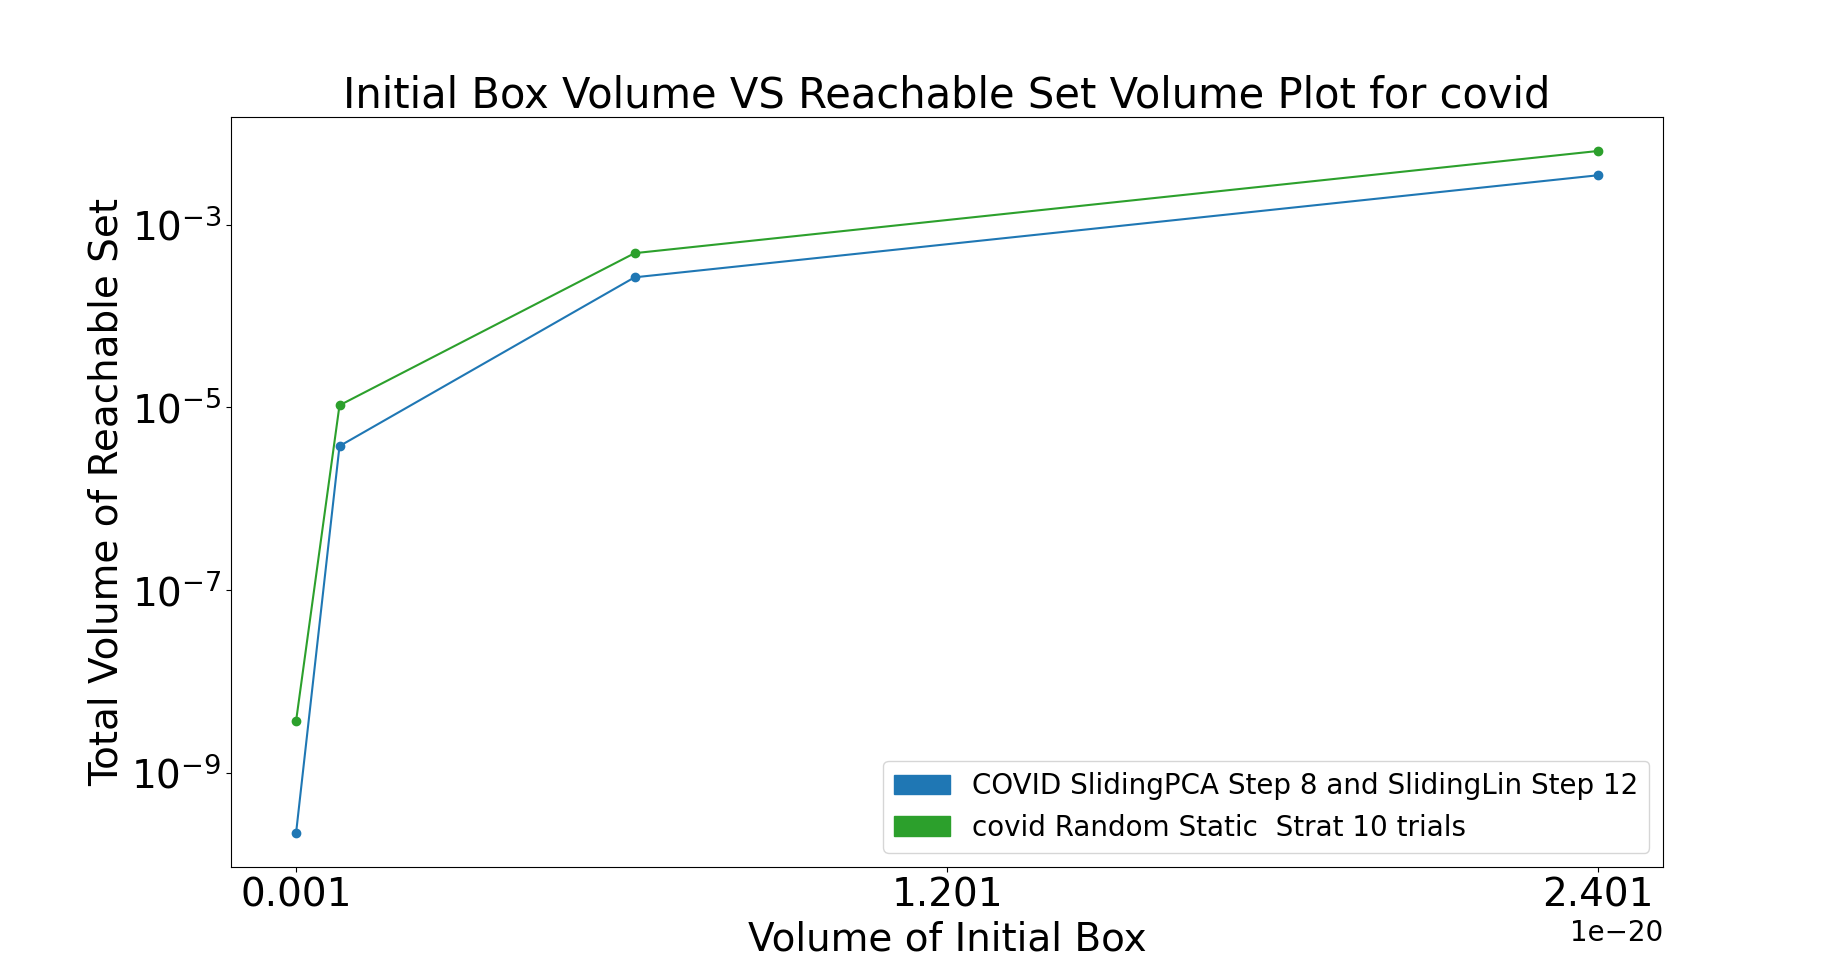
\includegraphics[width=\initvolwidth\textwidth, height=\initvolheight \textwidth]{figures/InitVolVSReachVol/CovidInitReachVolRanStrat.png}
  }

  \caption{Comparision between random static strategies and the best performing dynamic strategies as the volume of the initial set grows. The total reachable set volumes for random static strategies are averaged over ten trials for each system.}
  \label{fig:RanStaticStratComp}s
\end{figure}

